\documentclass[12pt]{book}

\usepackage{graphicx}
\usepackage[left=1.5in,right=1in]{geometry}
\makeatletter
\usepackage[colorlinks=true,allcolors=black]{hyperref}
\usepackage[cmex10]{amsmath}
\usepackage{amssymb}
\usepackage{array}
\usepackage{booktabs}
\usepackage{mathtools}
\usepackage{dirtree}
\usepackage{xcolor}
\usepackage{float}
\usepackage[justification=centering,font={rm,md,scriptsize}]{caption}
\usepackage{enumitem}
\usepackage{listings}
\usepackage{mathtools}

\def\baselinestretch{1.5}
\usepackage{fancyhdr}
\pagestyle{fancy}
\fancyhf{} 
\fancyfoot[C]{\thepage} 
\renewcommand{\headrulewidth}{0pt} 
\renewcommand{\footrulewidth}{0pt} 
\usepackage{xcolor}
\usepackage{sectsty}
\chapterfont{\color{blue}}
\sectionfont{\color{black}}
\newcounter{Chapcounter}
\newcommand\showmycounter{\addtocounter{Chapcounter}{1}\themycounter}
\counterwithin{enumi}{section}
\counterwithin{equation}{enumi}
\counterwithin{figure}{enumi}

\newcommand\figref{Fig.~\ref}

\setenumerate{label=\thesection.\arabic*}

\lstset{
  basicstyle=\ttfamily,
  columns=fullflexible,
  frame=single,
  breaklines=true,
  postbreak=\mbox{\textcolor{red}{$\hookrightarrow$}\space},
}

\providecommand{\mbf}{\mathbf}
\providecommand{\pr}[1]{\ensuremath{\Pr\left(#1\right)}}
\providecommand{\qfunc}[1]{\ensuremath{Q\left(#1\right)}}
\providecommand{\sbrak}[1]{\ensuremath{{}\left[#1\right]}}
\providecommand{\lsbrak}[1]{\ensuremath{{}\left[#1\right.}}
\providecommand{\rsbrak}[1]{\ensuremath{{}\left.#1\right]}}
\providecommand{\brak}[1]{\ensuremath{\left(#1\right)}}
\providecommand{\lbrak}[1]{\ensuremath{\left(#1\right.}}
\providecommand{\rbrak}[1]{\ensuremath{\left.#1\right)}}
\providecommand{\cbrak}[1]{\ensuremath{\left\{#1\right\}}}
\providecommand{\lcbrak}[1]{\ensuremath{\left\{#1\right.}}
\providecommand{\rcbrak}[1]{\ensuremath{\left.#1\right\}}}
\newcommand{\sgn}{\mathop{\mathrm{sgn}}}
\providecommand{\abs}[1]{\left\vert#1\right\vert}
\providecommand{\res}[1]{\Res\displaylimits_{#1}} 
\providecommand{\norm}[1]{\left\lVert#1\right\rVert}
\providecommand{\mtx}[1]{\mathbf{#1}}
\providecommand{\mean}[1]{E\left[ #1 \right]}
\providecommand{\fourier}{\overset{\mathcal{F}}{ \rightleftharpoons}}
\providecommand{\ztrans}{\overset{\mathcal{Z}}{ \rightleftharpoons}}
\providecommand{\system}{\overset{\mathcal{H}}{ \longleftrightarrow}}
\newcommand{\solution}{\noindent \textbf{Solution: }}
\newcommand{\cosec}{\,\text{cosec}\,}
\providecommand{\dec}[2]{\ensuremath{\overset{#1}{\underset{#2}{\gtrless}}}}
\newcommand{\myvec}[1]{\ensuremath{\begin{pmatrix}#1\end{pmatrix}}}
\newcommand{\mydet}[1]{\ensuremath{\begin{vmatrix}#1\end{vmatrix}}}
\providecommand{\gauss}[2]{\mathcal{N}\ensuremath{\left(#1,#2\right)}}
\newcommand*{\permcomb}[4][0mu]{{{}^{#3}\mkern#1#2_{#4}}}
\newcommand*{\perm}[1][-3mu]{\permcomb[#1]{P}}
\newcommand*{\comb}[1][-1mu]{\permcomb[#1]{C}}
\let\vec\mathbf

\begin{document}

\large\title{DIGITAL COMMUNICATION}
\author{GANGA GOPINATH\\
Roll No. FWC22050\\}
\date{December 2022}
\normalsize
\maketitle

\tableofcontents

\bigskip

\setcounter{page}{1}

\chapter{Two Dice}
\section{Sum of Independant Random Variables}
Two dice, one blue and one grey, are thrown at the same time.   The event defined by the sum of the two numbers appearing on the top of the dice can have 11 possible outcomes 2, 3, 4, 5, 6, 6, 8, 9, 10, 11 and 12.  A student argues that each of these outcomes has a probability $\frac{1}{11}$.  Do you agree with this argument?  Justify your answer.
\begin{enumerate}
\item  {\em The Uniform Distribution: }Let $X_i \in \cbrak{1,2,3,4,5,6}, i = 1,2,$ be the random variables representing the outcome for each die.  Assuming the dice to be fair, the probability mass function (pmf) is expressed as 
\begin{align}
\label{eq:dice_pmf_xi}
p_{X_i}(n) = \pr{X_i = n} = 
\begin{cases}
\frac{1}{6} & 1 \le n \le 6
\\
0 & otherwise
\end{cases}
\end{align}
The desired outcome is
\begin{align}
\label{eq:dice_xdef}
X &= X_1 + X_2,
\\
\implies X &\in \cbrak{1,2,\dots,12}
\end{align}
%
The objective is to show that
\begin{align}
p_X(n) \ne \frac{1}{11}
\label{eq:dice_wrong}
\end{align}
\begin{flushleft}
\textsc{solution:}
The python code which was used to generate the results can be shared.
\end{flushleft}
\begin{center}
\fcolorbox{red}{white}{\parbox{12.5cm}
{\href{https://github.com/Gangagopinath/ASSIGNMENT/tree/main/digitalcommunication/codes/1/1.1.1.py}
{/codes/1/1.1.1.py}}}
\end{center}
\item {\em Convolution: }
From \eqref{eq:dice_xdef},
\begin{align}
p_X(n) &= \pr{X_1 + X_2 = n} = \pr{X_1  = n -X_2}
\\
&= \sum_{k}^{}\pr{X_1  = n -k | X_2 = k}p_{X_2}(k)
\label{eq:dice_x_sum}
\end{align}%
after unconditioning.  $\because X_1$ and $X_2$ are independent,
\begin{multline}
\pr{X_1  = n -k | X_2 = k} 
\\
= \pr{X_1  = n -k} = p_{X_1}(n-k)
\label{eq:dice_x1_indep}
\end{multline}
From \eqref{eq:dice_x_sum} and \eqref{eq:dice_x1_indep},
\begin{align}
p_X(n) = \sum_{k}^{}p_{X_1}(n-k)p_{X_2}(k) = p_{X_1}(n)*p_{X_2}(n)
\label{eq:dice_x_conv}
\end{align}
where $*$ denotes the convolution operation. 
Substituting from \eqref{eq:dice_pmf_xi}
in \eqref{eq:dice_x_conv},
\begin{align}
p_X(n) = \frac{1}{6}\sum_{k=1}^{6}p_{X_1}(n-k)= \frac{1}{6}\sum_{k=n-6}^{n-1}p_{X_1}(k)
\label{eq:dice_x_conv_x1}
\end{align}
\begin{align}
\because p_{X_1}(k) &= 0, \quad k \le 1, k \ge 6.
\end{align}
From \eqref{eq:dice_x_conv_x1},
\begin{align}
p_X(n) &= 
\begin{cases}
0 & n < 1
\\
\frac{1}{6}\sum_{k=1}^{n-1}p_{X_1}(k) &  1 \le n-1 \le  6
\\
\frac{1}{6}\sum_{k=n-6}^{6}p_{X_1}(k) & 1 < n-6 \le 6
\\
0 & n > 12
\end{cases}
\label{eq:dice_x_conv_cond}
\end{align}
Substituting from \eqref{eq:dice_pmf_xi} in \eqref{eq:dice_x_conv_cond},
\begin{align}
p_X(n) &= 
\begin{cases}
0 & n < 1
\\
\frac{n-1}{36} &  2 \le n \le  7
\\
\frac{13-n}{36} & 7 < n \le 12
\\
0 & n > 12
\end{cases}
\label{eq:dice_x_conv_final}
\end{align}
satisfying \eqref{eq:dice_wrong}.
\begin{flushleft}
\textsc{solution:}
The python code which was used to generate the results can be shared.
\end{flushleft}
\begin{center}
\fcolorbox{red}{white}{\parbox{12.5cm}
{\href{https://github.com/Gangagopinath/ASSIGNMENT/tree/main/digitalcommunication/codes/1/1.1.2.py}
{/codes/1/1.1.2.py}}}
\end{center}
\item {\em The $Z$-transform: }
The $Z$-transform of $p_X(n)$ is defined as 
%\cite{proakis_dsp}
\begin{align}
P_X(z) = \sum_{n = -\infty}^{\infty}p_X(n)z^{-n}, \quad z \in \mathbb{C}
\label{eq:dice_xz}
\end{align}
From \eqref{eq:dice_pmf_xi} and \eqref{eq:dice_xz}, 
\begin{align}
P_{X_1}(z) =P_{X_2}(z) &= \frac{1}{6}\sum_{n = 1}^{6}z^{-n}
\\
&=\frac{z^{-1}\brak{1-z^{-6}}}{6\brak{1-z^{-1}}}, \quad \abs{z} > 1
\label{eq:dice_xiz}
\end{align}
upon summing up the geometric progression.  
\begin{align}
\because p_X(n) &= p_{X_1}(n)*p_{X_2}(n),
\\
P_X(z) &= P_{X_1}(z)P_{X_2}(z)
\label{eq:dice_xzprod_def}
\end{align}
The above property follows from Fourier analysis and is fundamental to signal processing.  
From \eqref{eq:dice_xiz} and \eqref{eq:dice_xzprod_def},
\begin{align}
P_X(z) &= \cbrak{\frac{z^{-1}\brak{1-z^{-6}}}{6\brak{1-z^{-1}}}}^2
\\
&= \frac{1}{36}\frac{z^{-2}\brak{1-2z^{-6}+z^{-12}}}{\brak{1-z^{-1}}^2}
\label{eq:dice_xzprod}
\end{align}
Using the fact that 
%\cite{proakis_dsp}
\begin{align}
p_X(n-k) &\system{Z}P_X(z)z^{-k},
\\
nu(n)&\system{Z} \frac{z^{-1}}{\brak{1-z^{-1}}^2}
\end{align}
after some algebra, it can be shown that
%{\tiny
\begin{multline}
\frac{1}{36}\lsbrak{\brak{n-1}u(n-1) - 2 \brak{n-7}u(n-7)}
\\
\rsbrak{ +\brak{n-13}u(n-13)}
\\
\system{Z}
\frac{1}{36}\frac{z^{-2}\brak{1-2z^{-6}+z^{-12}}}{\brak{1-z^{-1}}^2}
\label{eq:dice_xz_closed}
\end{multline}
%}

where 
\begin{align}
u(n) =
\begin{cases}
1 & n \ge 0
\\
0 & n < 0
\end{cases}
\end{align}

From \eqref{eq:dice_xz}, \eqref{eq:dice_xzprod} and \eqref{eq:dice_xz_closed}
\begin{multline}
p_{X}(n) = \frac{1}{36}\lsbrak{\brak{n-1}u(n-1) 
}
\\
\rsbrak{- 2 \brak{n-7}u(n-7)+\brak{n-13}u(n-13)}
\end{multline}
which is the same as \eqref{eq:dice_x_conv_final}.  Note that  \eqref{eq:dice_x_conv_final} can be obtained from \eqref{eq:dice_xz_closed} using contour integration as well.
\\
\textsc{solution:}
The python code which was used to generate the results can be shared.
\begin{figure}[!ht]
\centering
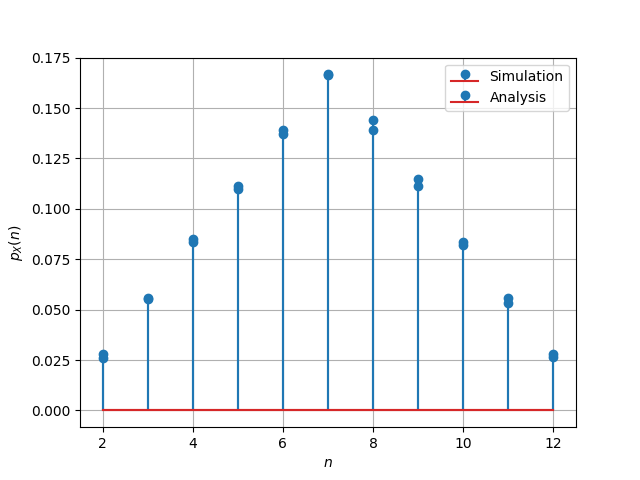
\includegraphics[width=\columnwidth]{./figs/1/1.1.3.png}
\caption{Plot of $p_X(n)$.  Simulations are close to the analysis. }
\label{fig:dice_1}
\end{figure}
\begin{center}
\fcolorbox{red}{white}{\parbox{12.5cm}
{\href{https://github.com/Gangagopinath/ASSIGNMENT/tree/main/digitalcommunication/codes/1/1.1.3.py}
{/codes/1/1.1.3.py}}}
\end{center}
\item 
The experiment of rolling the dice was simulated using Python for 10000 samples.  These were generated using Python libraries for uniform distribution. The frequencies for each outcome were then used to compute the resulting pmf, which  is plotted in Figure \ref{fig:dice}.  The theoretical pmf obtained in \eqref{eq:dice_x_conv_final} is plotted for comparison.  
%
\begin{figure}[H]
\centering

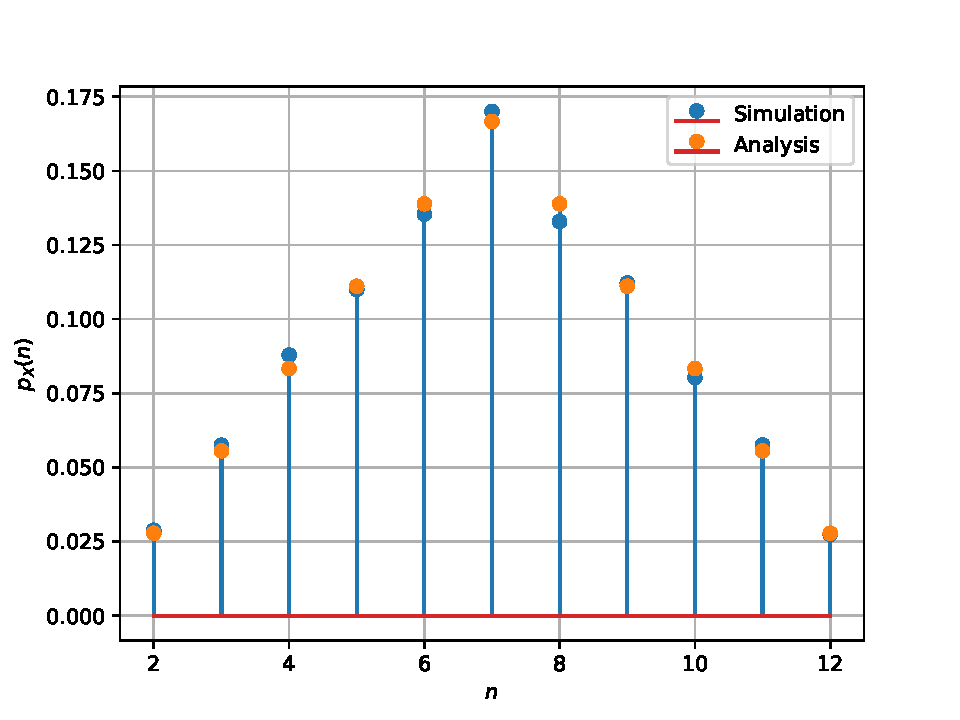
\includegraphics[width=\columnwidth]{./figs/1/1.1.4.pdf}
\caption{Plot of $p_X(n)$.  Simulations are close to the analysis. }
\label{fig:dice}
\end{figure}
\begin{flushleft}
The python code which was used to generate the results can be shared.
\end{flushleft}
\begin{center}
\fcolorbox{red}{white}{\parbox{12.5cm}
{\href{https://github.com/Gangagopinath/ASSIGNMENT/tree/main/digitalcommunication/codes/1/1.1.3.py}
{/codes/1/1.1.4.py}}}
\end{center}
\end{enumerate}

\chapter{Random Numbers}
\section{Uniform Random Numbers}
Let $U$ be a uniform random variable between 0 and 1.
\begin{enumerate}
\item Generate $10^6$ samples of $U$ using a C program and save into a file called uni.dat .
\label{prob:uni_gen}
\\
\solution Download the following files and execute the  C program.
\begin{center}
\fcolorbox{red}{white}{\parbox{12.5cm}
{\href{https://github.com/Gangagopinath/ASSIGNMENT/tree/main/digitalcommunication/codes/2/2.1.1.c}{/codes/coeffs.h}\\
{/codes/2/2.1.1.c}}}
\end{center}
\item
Load the uni.dat file into python and plot the empirical CDF of $U$ using the samples in uni.dat. The CDF is defined as
\begin{align}
F_{U}(x) = \pr{U \le x}
\end{align}
\\
\solution  The following code plots \figref{fig:uni_cdf}
\begin{center}
\fcolorbox{red}{white}{\parbox{12.5cm}
{\href{https://github.com/Gangagopinath/ASSIGNMENT/tree/main/digitalcommunication/codes/2/2.1.1.py}
{/codes/2/2.1.2.py}}}
\end{center}
\begin{figure}[H]
\centering
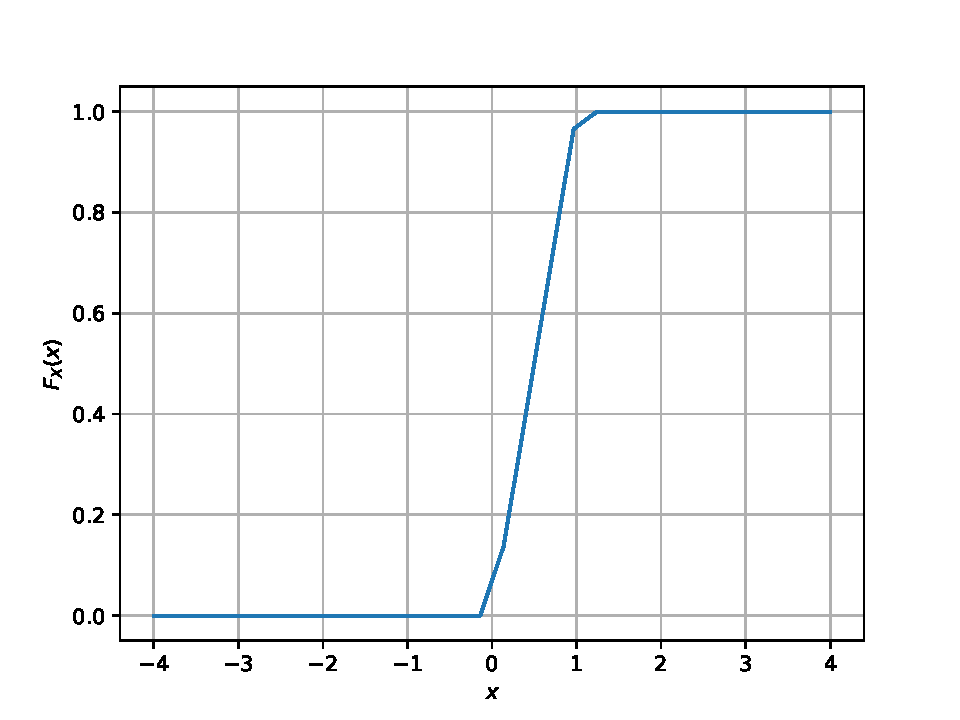
\includegraphics[width=\columnwidth]{./figs/2/2.1.2.pdf}
\caption{The CDF of $U$}
\label{fig:uni_cdf}
\end{figure}
\item
Find a  theoretical expression for $F_{U}(x)$.\\
\solution

\begin{align}
F_{U}(x) &= 
\begin{cases}
0 & x < a \\
\frac{x-a}{b-a} & a \leq x \leq b \\
1 & x \geq b
\end{cases}
\label{eq:cdf_of_random}
\end{align}
Substituting  a=0 and b=1. in \eqref{eq:cdf_of_random},
   
\begin{align}
F_{U}(x) &= 
\begin{cases}
0 & x < 0 \\
x& 0 \leq x \leq 1 \\
1 & x \geq 1
\end{cases}
\label{eq:uni_cdf}
\end{align}

\item
\label{prob:mean_var}
The mean of $U$ is defined as
%
\begin{equation}
E\sbrak{U} = \frac{1}{N}\sum_{i=1}^{N}U_i
\end{equation}
%
and its variance as
%
\begin{equation}
\text{var}\sbrak{U} = E\sbrak{U- E\sbrak{U}}^2 
\end{equation}
Write a C program to  find the mean and variance of $U$. \\
\solution
\begin{center}
\fcolorbox{red}{white}{\parbox{12.5cm}
{\href{https://github.com/Gangagopinath/ASSIGNMENT/tree/main/digitalcommunication/codes/2/2.1.4.c}
{/codes/2/2.1.4.c}\\
\href{https://github.com/Gangagopinath/ASSIGNMENT/tree/main/digitalcommunication/codes/2/uni.dat}
{/codes/2/uni.dat}}}
\end{center}
\item Verify your result theoretically given that
%
\begin{equation}
E\sbrak{U^k} = \int_{-\infty}^{\infty}x^kdF_{U}(x)
\end{equation}\\
\solution: The mean $\mu_X$ and variance $\sigma_X^2$ of a random variable $X$,are given by
\begin{align}
	\label{eq:mean_exp}
	\mu_X &= E\sbrak{X} = \int_{-\infty}^{\infty}xdF_{U}(x) \\
	\label{eq:var_exp}
	\sigma_X^2 &= E\sbrak{X^2} - \mu_X^2 = \int_{-\infty}^{\infty}x^2dF_{U}(x) - \mu_X^2\\
\end{align}
Substituting the CDF of $U$ from \eqref{eq:uni_cdf} in \eqref{eq:mean_exp} and \eqref{eq:var_exp}, we get
\large
\begin{center}
\begin{align*}
 Mean:
E\sbrak{X} & =\int_a^b x \cdot \frac{1}{b-a} dx&\\
&= \frac{b^2-a^2}{2} \cdot \frac{1}{b-a}& \\
&= \frac{(b-a)(b+a)}{2} \cdot \frac{1}{b-a}& \\
&= \frac{b+a}{2} &\\
Here \  a=0,b=1&\\
\mu&= \mathrm{E}[X]= \frac{1}{2} = 0.5\\
E\sbrak{X^2}&=\int_a^b x^2 \cdot \frac{1}{b-a} dx\\ &=\frac{b^3-a^3}{3} \cdot \frac{1}{b-a} \\ &=\frac{a^2+ab+b^2}{3}&\\
Variance:
\sigma^2 &=E\left(X^2\right)-[E(X)]^2\\
&=\frac{(a-b)^2}{12}&\\
\sigma^2=0.834
\end{align*}
\end{center}
\normalsize
theoretically calculated mean and variance are consistent with the result obtained from the problem \ref{prob:mean_var}
\end{enumerate}

\section{Central Limit Theorem}
\begin{enumerate}

\item
Generate $10^6$ samples of the random variable
%
\begin{equation}
X = \sum_{i=1}^{12}U_i -6
\end{equation}
%
using a C program, where $U_i, i = 1,2,\dots, 12$ are  a set of independent uniform random variables between 0 and 1
and save in a file called gauss.dat\\
\solution Download the following files and execute the  C program.
\begin{center}
\fcolorbox{red}{white}{\parbox{12.5cm}
{\href{https://github.com/Gangagopinath/ASSIGNMENT/tree/main/digitalcommunication/codes/2/2.2.1.c}
{/codes/2/2.2.1.c}\\
\href{https://github.com/Gangagopinath/ASSIGNMENT/tree/main/digitalcommunication/codes/2/Gauss.dat}
{/codes/2/Gauss.dat}}}
\end{center}
\item
Load Gauss.dat in python and plot the empirical CDF of $X$ using the samples in Gauss.dat. What properties does a CDF have?
\\
\solution The CDF of $X$ is plotted in \figref{fig:gauss_cdf}
\begin{figure}[H]
\centering
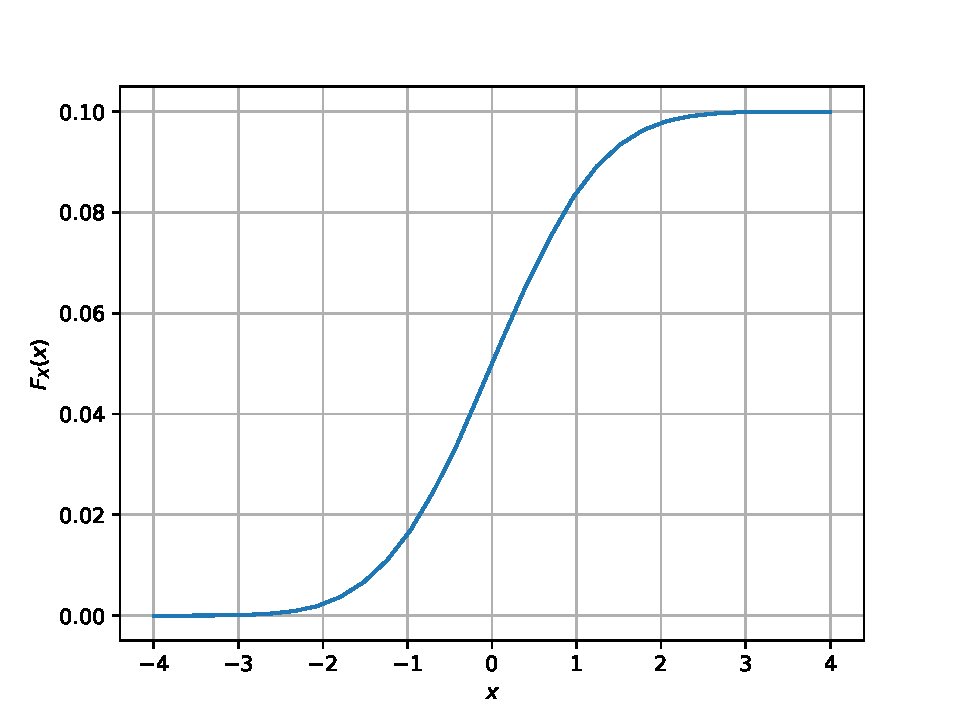
\includegraphics[width=\columnwidth]{./figs/2/2.2.2.pdf}
\caption{The CDF of $X$}
\label{fig:gauss_cdf}
\end{figure}
\textbf{Properties:}\\

\begin{itemize}
\item CDF is non-decreasing function 
\item Right continous.
\item $F_{max}(+\infty)=1$.
\item $F_{min}(-\infty)=0$.
%\item Let X be a continuous random variable. If the CDF $F(x)$ is continuous at
%any $ a \leq x \leq b $,then
%\begin{align}
\item $P[{a \leq x \leq b}] =F_{x}(b)-F_{x}(a) $
\item { $\frac{dF_X(x)}{dx} \ge 0$}
\end{itemize}
\item
Load Gaussian.dat in python and plot the empirical PDF of $X$ using the samples in Gaussian.dat. The PDF of $X$ is defined as
\begin{align}
p_{X}(x) = \frac{d}{dx}F_{X}(x)
\end{align}
What properties does the PDF have?
\\
\solution The PDF of $X$ is plotted in Fig. \ref{fig:gauss_pdf} using the code below
\begin{figure}[H]
\centering
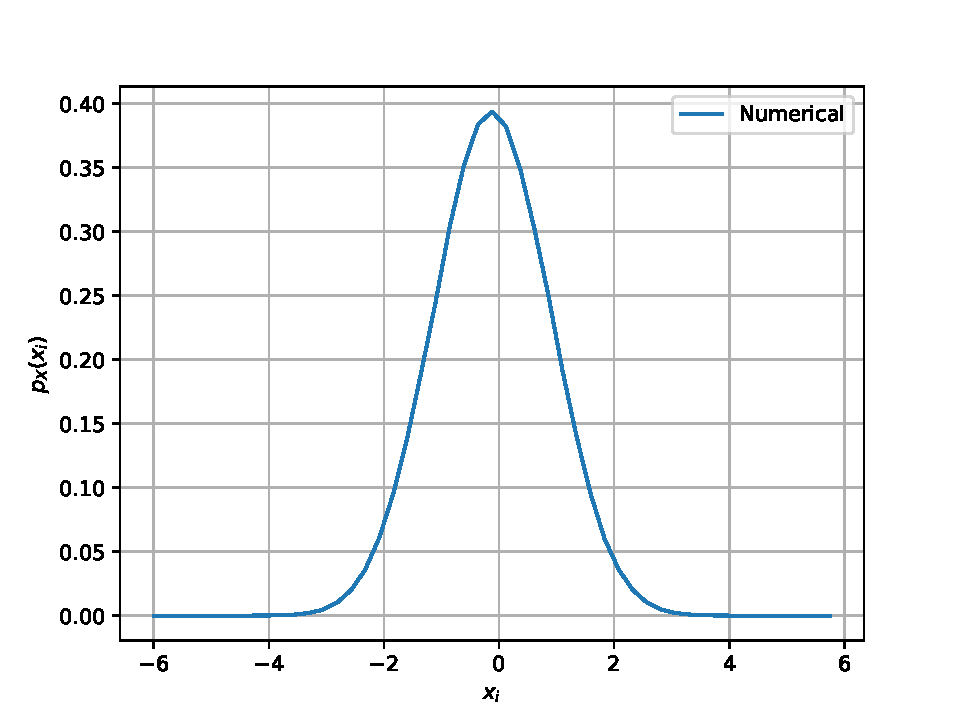
\includegraphics[width=\columnwidth]{./figs/2/2.2.3.pdf}
\caption{The PDF of $X$}
\label{fig:gaus_pdf}
\end{figure}
\begin{center}
\fcolorbox{red}{white}{\parbox{12.5cm}
{\href{https://github.com/Gangagopinath/ASSIGNMENT/tree/main/digitalcommunication/codes/2/2.2.3.py}
{/codes/2/2.2.3.py}\\
\href{https://github.com/Gangagopinath/ASSIGNMENT/tree/main/digitalcommunication/codes/2/Gauss.dat}
{/codes/2/Gauss.dat}}}
\end{center}
\textbf{Properties} : 
\begin{itemize}
\item $f_X(x) \ge 0 ,{-\infty \leq x \leq \infty}$
\item $\int_{-\infty}^{\infty} f_X(x) \,dx = 1$
\item $P[{x_1 \leq X \leq x_2}] =\int_{x_1}^{x_2} f_X(x) \,dx $
\end{itemize}
\item Find the mean and variance of $X$ by writing a C program.\\
\solution : Download the following files and run the  C program.
\begin{center}
\fcolorbox{red}{white}{\parbox{12.5cm}
{\href{https://github.com/Gangagopinath/ASSIGNMENT/tree/main/digitalcommunication/codes/2/2.2.1.c}
{/codes/2/2.2.1.c}\\
\href{https://github.com/Gangagopinath/ASSIGNMENT/tree/main/digitalcommunication/codes/2/Gauss.dat}
{/codes/2/Gauss.dat}}}
\end{center}
\item Given that 
\begin{align}
p_{X}(x) = \frac{1}{\sqrt{2\pi}}\exp\brak{-\frac{x^2}{2}}, -\infty < x < \infty,
\end{align}
repeat the above exercise theoretically.\\
\solution
\begin{align}
Mean(\mu) = E(X)\\
E(X)= \frac{1}{\sqrt{2\pi}} \int_{-\infty}^{\infty} x e^{-\frac{x^2}{2}}dx=0 \\
Variance( \sigma^2) =  E\brak X^2 - E^2\brak X 
\end{align}
\begin{align}
    E\brak{X^2}&= \frac{1}{\sqrt{2\pi}}\int_{-\infty}^{\infty} x^2
e^ {-\frac{x^2}{2}} dx \quad \brak{even function}\\
    &= \frac{2}{\sqrt{2\pi}} \int_{0}^{\infty} x^2 e^{-\frac{x^2}{2}} dx\\
    &= \frac{2}{\sqrt{2\pi}}\int_{0}^{\infty}\sqrt{2y}e^{-y} dy \quad\brak{ \frac{x^2}{2}= y}\\
        &= \frac{2}{\sqrt{\pi}} \int_{0}^{\infty} e^{-y} y^{\frac{1}{2}} dy\\
    &= \frac{2}{\sqrt{\pi}} \int_{0}^{\infty} e^{-y} y^{(\frac{1}{2}+1)-1} dy \quad\brak{\Gamma(x) = \int_{0}^{\infty} z^{x-1} \cdot e^{-z} , dz}\\
    &= \frac{2}{\sqrt{\pi}} \Gamma\brak{{\frac{1}{2}+1}}\\
    &= \frac{1}{\sqrt{\pi}}\Gamma\brak{\frac{1}{2}} \\
    &= 1
\end{align}
where 
\begin{align}
\Gamma\brak{\frac{1}{2}}=\sqrt{\pi}
\end{align}
%
Thus, the  variance is
\begin{align}
    \sigma^2 =  E\brak X^2 - E^2\brak X = 1
\end{align}
numerical and theoretical  plots as shown in fig.\ref{fig:gauss_pdf}
\begin{center}
\fcolorbox{red}{white}{\parbox{12.5cm}
{\href{https://github.com/Gangagopinath/ASSIGNMENT/tree/main/digitalcommunication/codes/2/2.2.5.py}
{/codes/2/2.2.5.py}\\
\href{https://github.com/Gangagopinath/ASSIGNMENT/tree/main/digitalcommunication/codes/2/Gauss.dat}
{/codes/2/Gauss.dat}}}
\end{center}
\begin{figure}
\centering
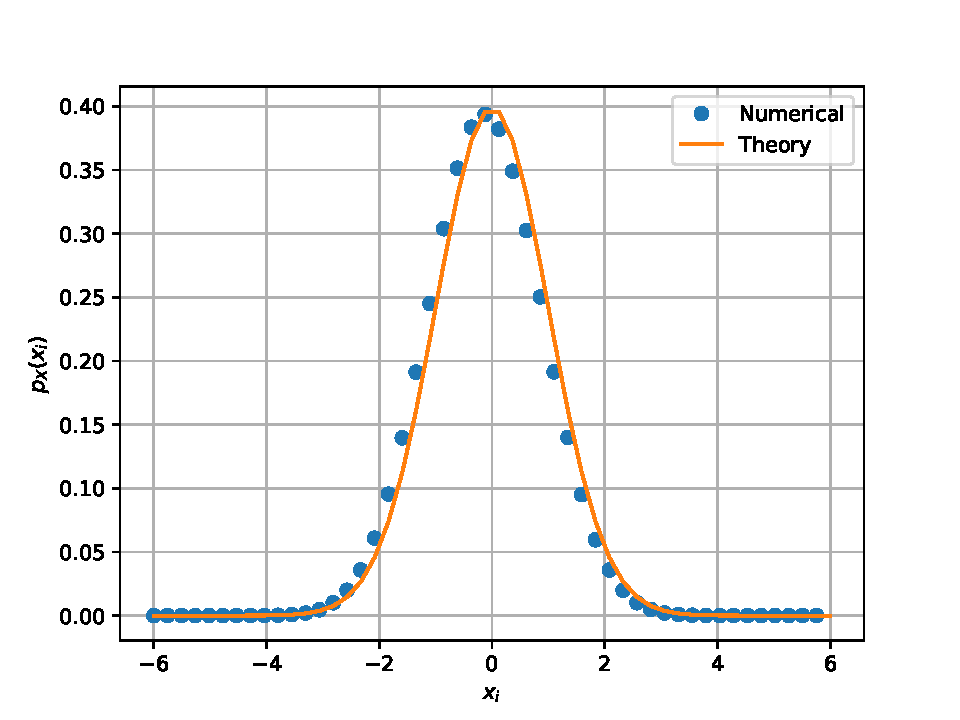
\includegraphics[scale=0.5]{./figs/2/2.2.4.pdf}  
\caption{The PDF of $p\brak{x}$}
\label{fig:gauss_pdf}
\end{figure}
\end{enumerate}
\section{From Uniform to Other}
\begin{enumerate}
%
\item
Generate samples of 
%
\begin{equation}
V = -2\ln\brak{1-U}
\end{equation}
and plot its CDF. \\
\solution:
Code loads the samples from the v.dat file generated and plot the cdf of $V$ 

\begin{center}
\fcolorbox{red}{white}{\parbox{12.5cm}
{\href{https://github.com/Gangagopinath/ASSIGNMENT/tree/main/digitalcommunication/codes/2/2.3.1.c}
{/codes/2/2.3.1.c}\\
\href{https://github.com/Gangagopinath/ASSIGNMENT/tree/main/digitalcommunication/codes/2/2.3.1.py}
{/codes/2/2.3.1.py}}}
\end{center}
\begin{figure}[H]
\centering
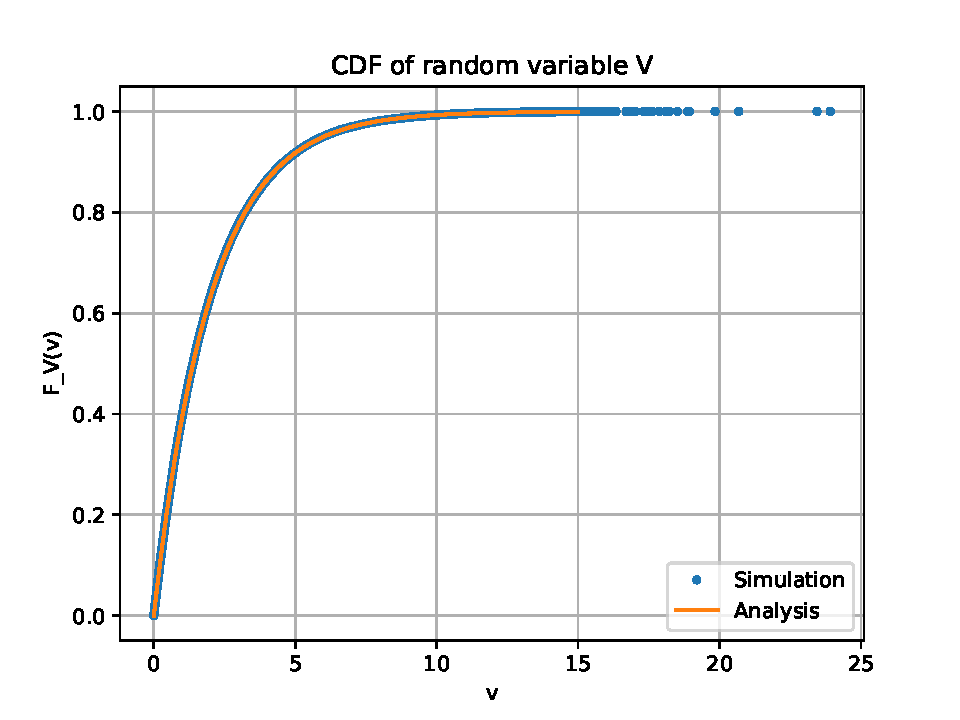
\includegraphics[scale=0.5]{./figs/2/2.3.1.pdf}  
\caption{The CDF of $V$}
\label{fig:log_uni_cdf}
\end{figure}
\item Find a theoretical expression for $F_V(x)$.
\begin{flalign}
	F_V(x) &= P(V \le x)&\\
	&= P(-2\ln\brak{1-U} \le x)&\\
	&= P(\ln\brak{1-U} \geq - \frac{x}{2})\\
	&= P(1-U \geq e^{\frac{-x}{2}})&\\
	&= P(U \le 1 - e^{\frac{-x}{2}})&\\
	&= F_U(1 - e^{\frac{-x}{2}})
\end{flalign}
\end{enumerate}


\section{Triangular Distribution}
\begin{enumerate}
\item Generate 
	\begin{align}
		T = U_1+U_2
	\end{align}\\
\solution Download the following files and execute the  C program.
\begin{center}
\fcolorbox{red}{white}{\parbox{12.5cm}
{\href{https://github.com/Gangagopinath/ASSIGNMENT/tree/main/digitalcommunication/codes/2/2.4.1.c}
{/codes/2/2.4.1.c}}}
\end{center}
\item Find the CDF of $T$.\\
\solution Loading the samples from tri.dat in python, the CDF is plotted in \figref{fig:tri_cdf} 
\begin{figure}[H]
\centering
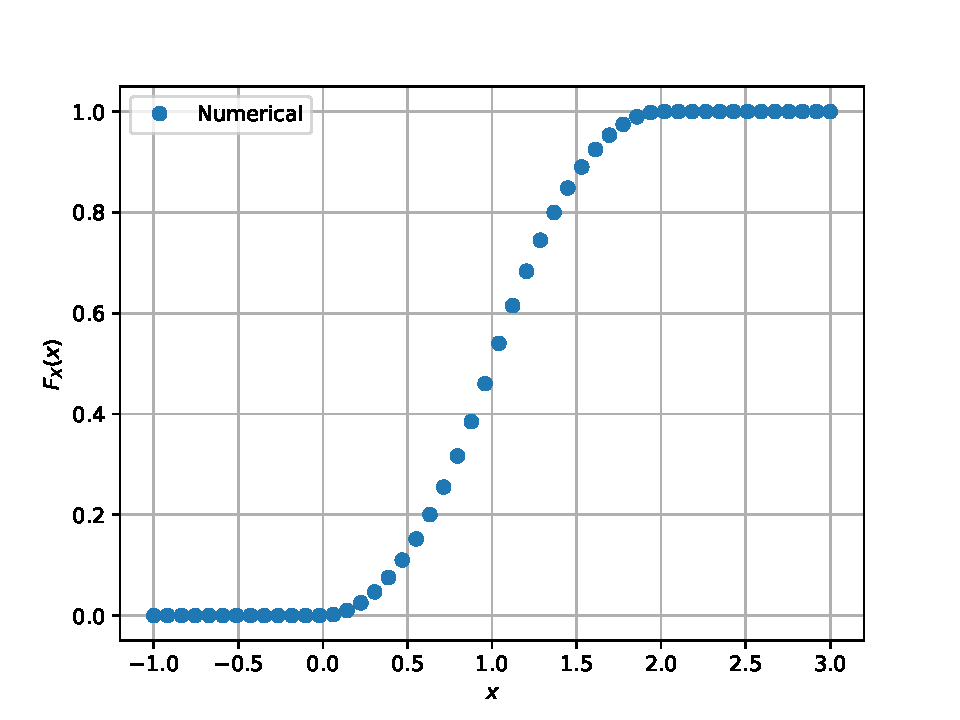
\includegraphics[width=\columnwidth]{./figs/2/2.4.2.pdf}
\caption{The CDF of $T$}
\label{fig:tri_cdf}
\end{figure}
\item Find the PDF of $T$.\\
\solution The PDF of $T$ is plotted in \figref{fig:tri_pdf} using the code below
\solution Download the following files and execute the  C program.
\begin{center}
\fcolorbox{red}{white}{\parbox{12.5cm}
{\href{https://github.com/Gangagopinath/ASSIGNMENT/tree/main/digitalcommunication/codes/2/2.4.3.py}
{/codes/2/2.4.3.py}}}
\end{center}
\begin{figure}[H]
\centering
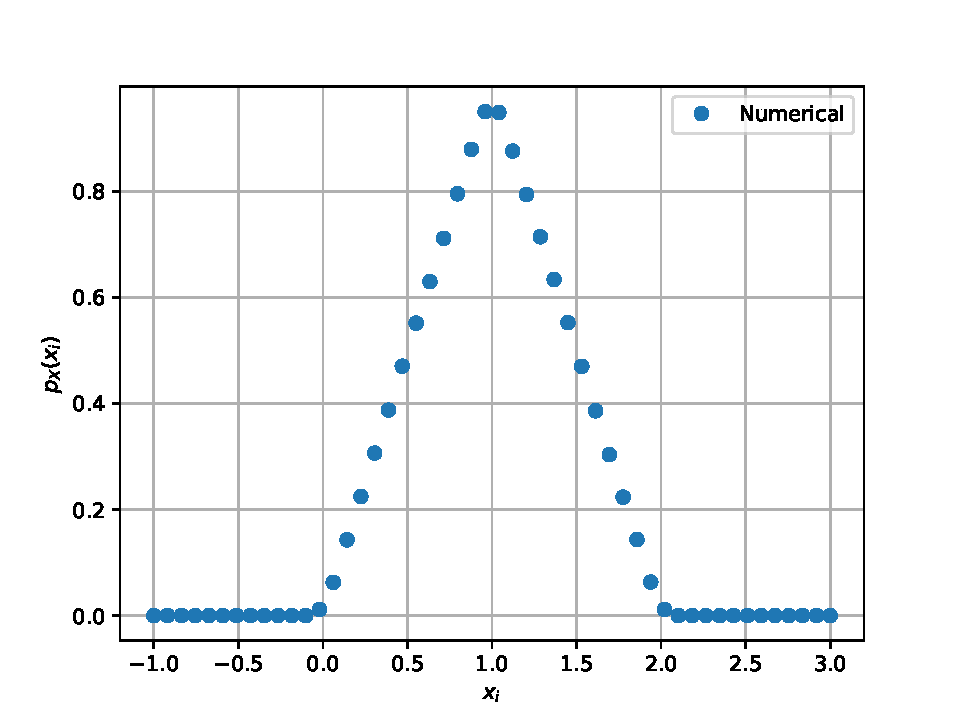
\includegraphics[width=\columnwidth]{./figs/2/2.4.3.pdf}
\caption{The PDF of $T$}
\label{fig:tri_pdf}
\end{figure}
\item Find the theoretical expressions for the PDF and CDF of $T$.\\
\solution 
CDF ($F_T(x)$) of a triangular distribution  is 
\begin{align}
F_{T}(x) &= 
\begin{cases}
0 & x \leq a \\
\frac{(x-a)^2}{(b-a)(c-a)} & a < x \leq c \\
1-\frac{(b-x)^2}{(b-a)(c-a)} & c < x \leq b\\
1 & x > b
\end{cases}
\end{align}
PDF ($p_T(x)$) of a triangular distribution is
\begin{align}
p_{T}(x) = \frac{d}{dx}F_{U}(x)
\end{align}
\begin{align}
p_{U}(x) &= 
\begin{cases}
0 & x \leq a \\
\frac{2(x-a)}{(b-a)(c-a)} & a < x \leq c \\
\frac{2(b-x)}{(b-a)(c-a)} & c < x \leq b\\
0 & x > b
\end{cases}
\end{align}
\item Verify your results through a plot. \\
\solution : Compare using the Python codes provided below and the corresponding plots shown \figref{fig:trii_cdf} and \figref{fig:trii_pdf}
\begin{center}
\fcolorbox{red}{white}{\parbox{12.5cm}
{\href{https://github.com/Gangagopinath/ASSIGNMENT/tree/main/digitalcommunication/codes/2/2.4.4a.py}
{/codes/2/2.4.4a.py}\\
\href{https://github.com/Gangagopinath/ASSIGNMENT/tree/main/digitalcommunication/codes/2/2.4.4b.py}
{/codes/2/2.4.4b.py}}}
\end{center}
\begin{figure}[H]
\centering
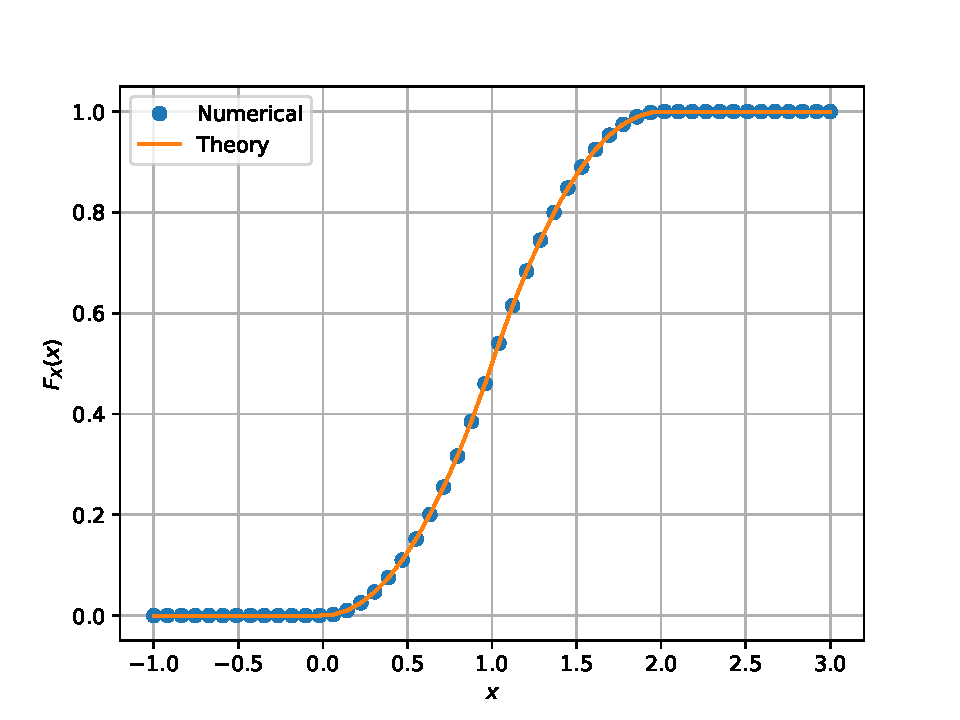
\includegraphics[width=110mm,scale=1]{./figs/2/2.4.4a.pdf}
\caption{The CDF of $T$}
\label{fig:trii_cdf}
\end{figure}
\begin{figure}[H]
\centering
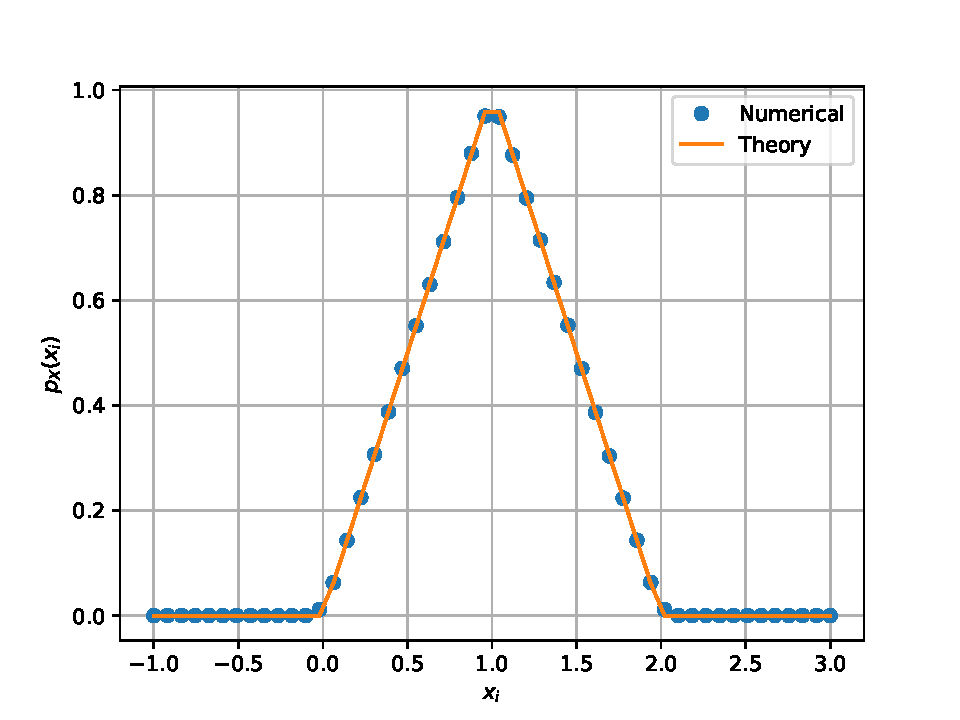
\includegraphics[width=\columnwidth]{./figs/2/2.4.4b.pdf}
\caption{The PDF of $T$}
\label{fig:trii_pdf}
\end{figure}
\end{enumerate}
\chapter{Maximum Likelihood Detection: BPSK}
\section{Maximum Likelihood}
\begin{enumerate}
\item Generate equiprobable $X \in \cbrak{1,-1}$.\\
\solution $X$ can be generated in python using the  code section,
\begin{center}
\fcolorbox{red}{white}{\parbox{12.5cm}
{\href{https://github.com/Gangagopinath/ASSIGNMENT/tree/main/digitalcommunication/codes//3.1.1.py}
{/codes/3/3.1.1.py}}}
\end{center}
\item Generate 
\begin{equation}
Y = AX+N,
\end{equation}
		where $A = 5$ dB,  and $N \sim \gauss{0}{1}$.\\
\solution $Y$ can be generated in python using the below code section,
\begin{center}
\fcolorbox{red}{white}{\parbox{12.5cm}
{\href{https://github.com/Gangagopinath/ASSIGNMENT/tree/main/digitalcommunication/codes//3.1.2.py}
{/codes/3/3.1.2.py}}}
\end{center}
\item Plot $Y$ using a scatter plot.\\
\solution The scatter plot of $Y$ is plotted in \figref{fig:bpsk_scatter} using the below code,
\begin{center}
\fcolorbox{red}{white}{\parbox{12.5cm}
{\href{https://github.com/Gangagopinath/ASSIGNMENT/tree/main/digitalcommunication/codes//3.1.3.py}
{/codes/3/3.1.3.py}}}
\end{center}
\begin{figure}[H]
\centering
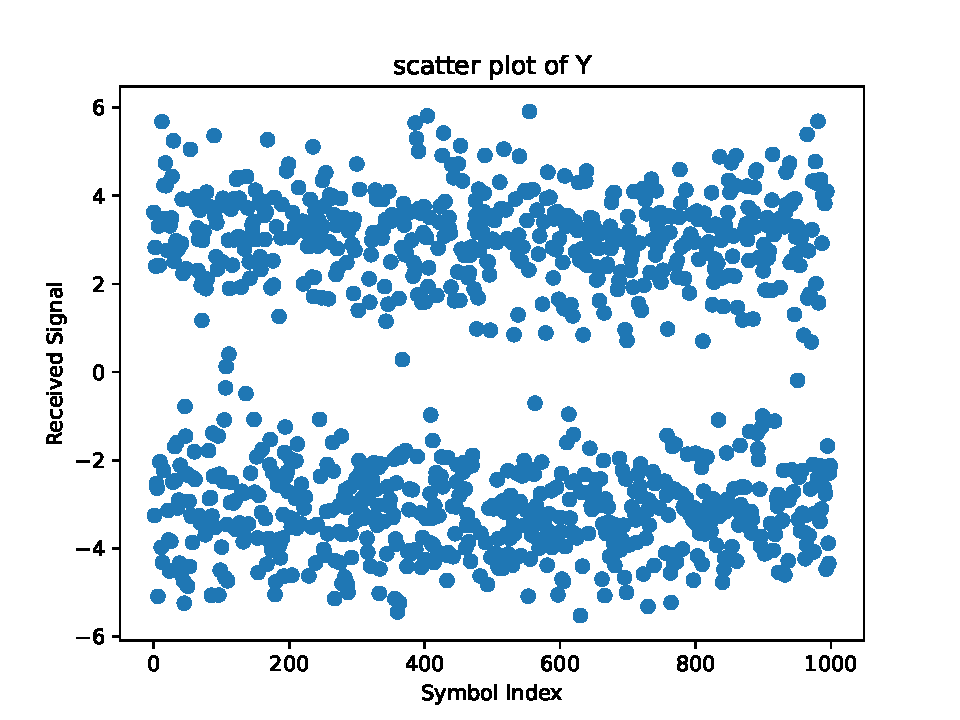
\includegraphics[width=\columnwidth]{./figs/3/3.1.3.pdf}
\caption{Scatter plot of $Y$}
\label{fig:bpsk_scatter}
\end{figure}
\item Guess how to estimate $X$ from $Y$.\\
\solution
\begin{equation}
y \dec{1}{-1} 0
\label{eq:bpsk_decision}
\end{equation}
\item
\label{ml-ch4_sim}
Find 
\begin{equation}
	P_{e|0} = \pr{\hat{X} = -1|X=1}
\end{equation}
and 
\begin{equation}
	P_{e|1} = \pr{\hat{X} = 1|X=-1}
\end{equation}\\
\solution The probability of error can be calculated using the decision rule in \eqref{eq:bpsk_decision},

\begin{flalign*}
	P_{e|0} &= \pr{\hat{X} = -1|X=1}&\\
	&= \pr{Y < 0|X=1}&\\
	&= \pr{AX + N < 0|X=1}&\\ 
	&= \pr{N<-AX|X=1}&\\
	&= \pr{N < -A }&\\
	&= Q(-A)
\end{flalign*}

\begin{flalign*}
P_{e|1} &= \pr{\hat{X} = 1|X=-1}&\\
&=\pr{Y>0|X=-1}&\\
&=\pr{AX+N>0|X=-1}&\\
&=\pr{N>-AX|X=-1}&\\
&=\pr{N>A}&\\  
&=Q(A)
\end{flalign*}


where,$N \sim \gauss{0}{1}$\\
\begin{align}
 \therefore \pr{N>A}=\pr{N<-A}\\
 P_{e|0}=P_{e|1} \label{eq:equi_prob}
\end{align}
\eqref{eq:equi_prob}is known as the symmetry property of the Gaussian distribution.
\item Find $P_e$ assuming that $X$ has equiprobable symbols.\\
 \solution \begin{align}
	P_e &= \pr{X=1}P_{e|1} + \pr{X=-1}P_{e|0}& \label{eq:Pe_of_X}
	\end{align}
	\text{given $X$ is equiprobable}\\
	\begin{align}
	P_e &= \frac{1}{2}P_{e|1} + \frac{1}{2}P_{e|0}
\end{align}
Substituting from \eqref{eq:equi_prob}
\begin{equation}
	P_e = \pr{N > A}
\end{equation}
Given a random varible $X \sim \gauss{0}{1}$ the Q-function can be expressed as
\begin{align}
	Q(x) &= \pr{X > x}\\
	\label{eq:q_func_integral}
	Q(x) &= \frac{1}{\sqrt{2\pi}} \int_x^\infty \exp\left(-\frac{t^2}{2}\right) \, dt.
\end{align}
By using the Q-function, $P_e$ can be expressed in terms of Q-function
\begin{equation}
	P_e = Q(A)
\end{equation} 
\item
Verify by plotting  the theoretical $P_e$ with respect to $A$ from 0 to 10 dB.\\
\solution 
in figure \ref{fig:bpsk_pe_snr} both the theoretical and numerical estimations from generated samples of Y are plotted using this code
\begin{center}
\fcolorbox{red}{white}{\parbox{12.5cm}
{\href{https://github.com/Gangagopinath/ASSIGNMENT/tree/main/digitalcommunication/codes//3.1.7.py}
{/codes/3/3.1.7.py}}}
\end{center}
\begin{figure}[H]
\centering
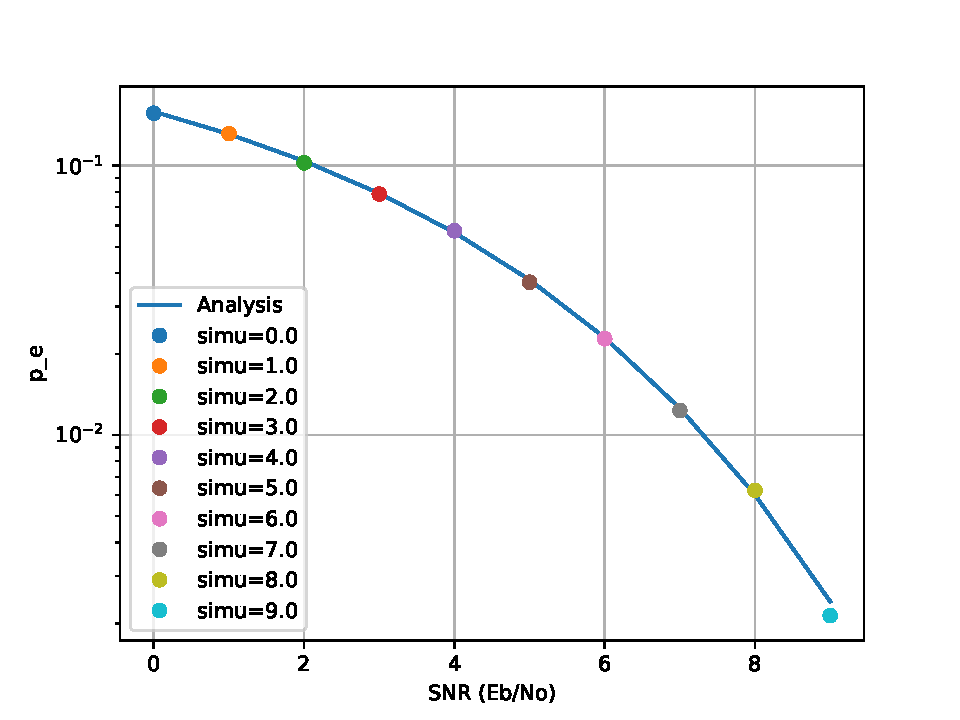
\includegraphics[width=\columnwidth]{./figs/3/3.1.7.pdf}
\caption{Scatter plot of $Y$}
\label{fig:bpsk_pe_snr}
\end{figure}
\item Now, consider a threshold $\delta$  while estimating $X$ from $Y$. Find the value of $\delta$ that maximizes the theoretical $P_e$.\\
\label{prob:bpsk_delta_equi}
\solution Given the decision rule, 
\begin{equation}
y \dec{1}{-1} \delta
\label{eq:bpsk_decision_delta}
\end{equation}
\begin{flalign*}
	P_{e|0} &= \pr{\hat{X} = -1|X=1}&\\
	&= \pr{Y < \delta|X=1}&\\
	&= \pr{AX + N < \delta|X=1}&\\ 
	&= \pr{A + N < \delta}&\\
	&= \pr{N < -A + \delta}&\\
	&= \pr{N > A - \delta}&\\
	&= Q(A-\delta)
\end{flalign*}
\begin{flalign*}
	P_{e|1} &= \pr{\hat{X} = 1|X=-1}&\\
	&= \pr{Y > \delta|X=-1}&\\
	&= \pr{AX + N > \delta|X=-1}&\\ 
	&= \pr{N > A + \delta}&\\
	&= Q(A+\delta)
\end{flalign*}

The overall $P_e$ is the average of these two probabilities, which is given by:
\begin{flalign}
P_e = \frac{1}{2}Q(A+\delta) + \frac{1}{2}Q(A-\delta)
\end{flalign}

Differentiating this equation with respect to $\delta$ and equating it to 0, we get:
\begin{flalign}
\frac{\partial P_e}{\partial \delta} = \frac{1}{2}\frac{\partial Q(A+\delta)}{\partial \delta} - \frac{1}{2}\frac{\partial Q(A-\delta)}{\partial \delta} = 0 &\\ \vspace{15mm}
\frac{\partial Q(A+\delta)}{\partial \delta} - \frac{\partial Q(A-\delta)}{\partial \delta} = 0
\end{flalign}
And by the Leibniz's rule:
\begin{flalign}
\frac{d}{dx} \int_{f(x)}^{g(x)}h(t,x)dt = h(g(x),x)g'(x) - h(f(x),x)f'(x)
\end{flalign}
We get
\begin{flalign}
\frac{\frac{\partial}{\partial \delta} \int_{A+\delta}^{\infty}e^{-\frac{u^2}{2}}du - \frac{\partial}{\partial \delta} \int_{A-\delta}^{\infty}e^{-\frac{u^2}{2}}du}{\partial \delta} = 0 \\
\frac{e^{-\frac{(A+\delta)^2}{2}}}{\partial \delta} - \frac{e^{-\frac{(A-\delta)^2}{2}}}{\partial \delta} = 0
\end{flalign}
Solving for $\delta$ we get
\begin{flalign}
e^{-\frac{(A+\delta)^2}{2}} - e^{-\frac{(A-\delta)^2}{2}} = 0\\
\frac{e^{-\frac{(A+\delta)^2}{2}}}{e^{-\frac{(A-\delta)^2}{2}}} = 1\\
e^{-\frac{(A+\delta)^2 - (A-\delta)^2}{2}} = 1\\
e^{-2A\delta} = 1\\
\ln(e^{-2A\delta}) = \ln(1)\\
-2A\delta = 0\\
\delta = 0
\end{flalign}

\item Repeat the above exercise when 
	\begin{align}
		p_{X}(0) = p
	\end{align}
	\solution


Given $X$ is not equiprobable, $P_e$ is given by,

\begin{align}
P_e &= (1-p)P_{e|1} + pP_{e|0}\ \\
&= (1-p)Q(A+\delta) + pQ(A-\delta)
\end{align}

Where $Q(x)$ is the Q-function
\begin{align}
Q(x)=\frac{1}{\sqrt{2\pi}}\int_{x}^{\infty}e^{-\frac{u^2}{2}}du
\end{align}
\begin{align}
P_e = k((1-p)\int_{A+\delta}^\infty \exp^{-\frac{u^2}{2}} du +
p\int_{A-\delta}^\infty \exp^{-\frac{u^2}{2}} du
\end{align}

where $k$ is a constant.

we differentiate the above expression with respect to $\delta$ and equate to zero,

\begin{align*}
\frac{\partial P_e}{\partial \delta} &== k((1-p)\frac{\partial}{\partial \delta}\int_{A+\delta}^\infty \exp^{\left(-\frac{u^2}{2}\right)} , du - p\frac{\partial}{\partial \delta}\int_{A-\delta}^\infty \exp^{\left(-\frac{u^2}{2}\right)} , du) = 0\\
&=k((1-p)\exp{-\frac{(A+\delta)^2}{2}} - p\exp{-\frac{(A-\delta)^2}{2}} = 0
\end{align*}

Dividing both sides by $(1-p)\exp^{-\frac{(A+\delta)^2}{2}}$ we get

\begin{align*}
\frac{\exp\-\frac{(A+\delta)^2}{2}}{\exp-\frac{(A-\delta)^2}{2}} = \frac{p}{(1-p)}
\end{align*}

Taking $\ln$ on both sides

\begin{align*}
\ln\left(\frac{\exp\left(-\frac{(A+\delta)^2}{2}\right)}{\exp\left(-\frac{(A-\delta)^2}{2}\right)}\right) = \ln\left(\frac{p}{(1-p)}\right)
\end{align*}

Using the properties of $\ln$ and $\exp$, we can simplify the above as

\begin{align*}
\ln\left(\exp\left(-\frac{(A+\delta)^2}{2}\right)\exp\left(\frac{(A-\delta)^2}{2}\right)\right) = \ln\left(\frac{p}{(1-p)}\right)
\end{align*}

Rearranging and using the properties of exponential function
\begin{align*}
\ln\left(\exp\left(-\frac{(A+\delta)^2}{2}+\frac{(A-\delta)^2}{2}\right)\right) = \ln\left(\frac{p}{(1-p)}\right)
\end{align*}

\begin{align*}
\ln\left(\exp\left(-2A\delta\right)\right) = \ln\left(\frac{p}{(1-p)}\right)
\end{align*}

Solving for $\delta$
\begin{align*}
-2A\delta = \ln\left(\frac{p}{(1-p)}\right)
\end{align*}

\begin{align*}
\delta = \frac{1}{2A}\ln\left(\frac{p}{(1-p)}\right)
\end{align*}

Finally taking the exponential of both sides
\begin{align*}
\delta = \frac{1}{2A}\log\left(\frac{1}{p}-1\right)
\end{align*}

Therefore, the optimal value of $\delta$  is given by  
\begin{align*}
\delta = \frac{1}{2A}\log\left(\frac{1}{p}-1\right)
\end{align*}
\iffalse
\item Repeat the above exercise using the MAP criterion.\\
\solution
\begin{center}
\fcolorbox{red}{white}{\parbox{12.5cm}
{\href{https://github.com/Gangagopinath/ASSIGNMENT/tree/main/digitalcommunication/codes/3/3.1.9.py}
{/codes/3/3.1.9.py}}}
\end{center}
\begin{figure}[H]
\centering
\includegraphics[width=\columnwidth]{./figs/3/3.1.*.pdf}
\caption{$p_X(X=x_i)p_Y(y|x=x_i)$ versus $y$ plot for $X \in \{-1,1\}$}
\label{fig:bpsk_map_density}
\end{figure}
\fi
\end{enumerate}

\chapter{Transformation of Random Variables}
\section{Gaussian to Other}
\begin{enumerate}
\item
Let $X_1 \sim  \gauss{0}{1}$ and $X_2 \sim  \gauss{0}{1}$. Plot the CDF and PDF of
%
\begin{equation}
V = X_1^2 + X_2^2
\end{equation}\\
\solution The CDF and PDF of $V$ are plotted in \figref{fig:chisq_cdfpdf}  using the below code
\begin{center}
\fcolorbox{red}{white}{\parbox{12.5cm}
{\href{https://github.com/Gangagopinath/ASSIGNMENT/tree/main/digitalcommunication/codes/4/4.1.1.py}
{/codes/4/4.1.1.py}}}
\end{center}
\begin{figure}[H]
\centering
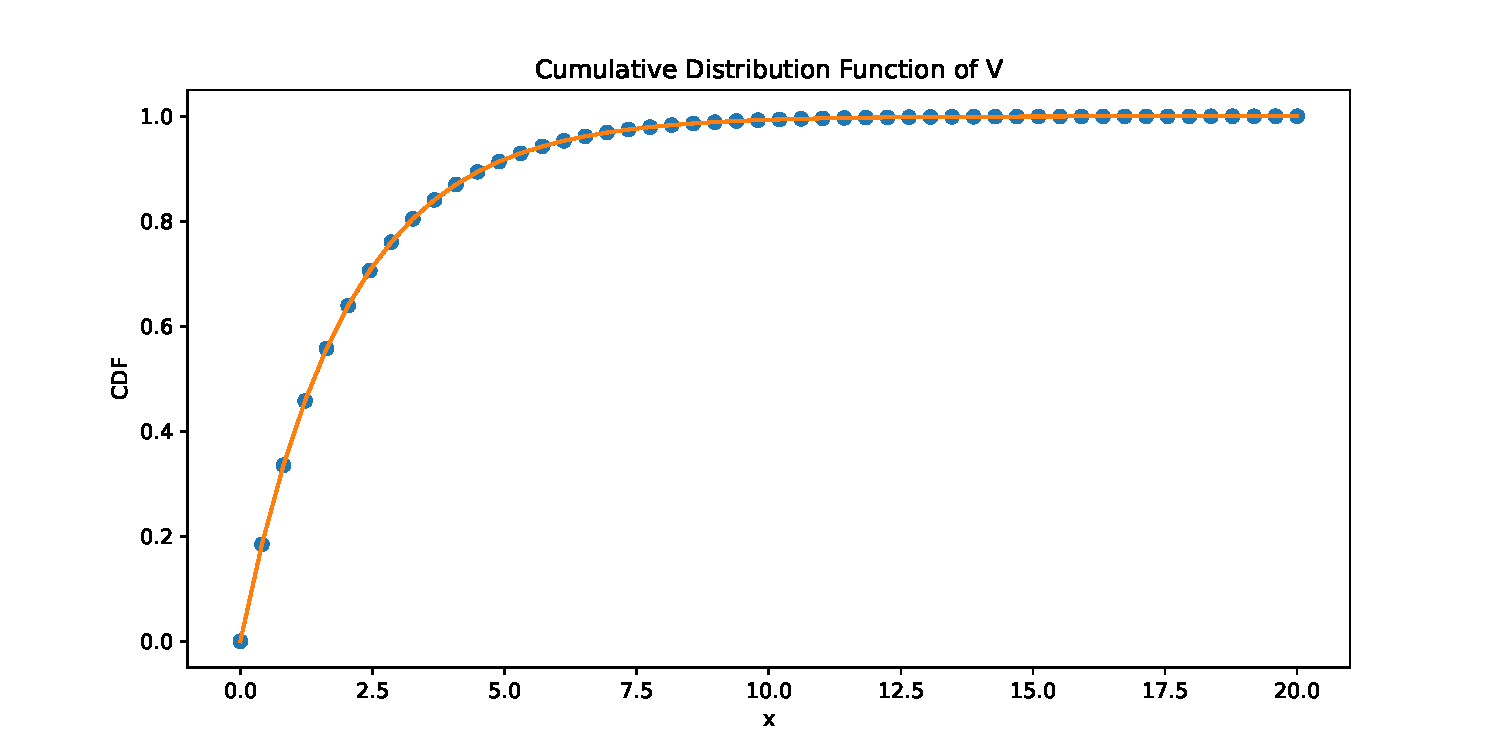
\includegraphics[width=\columnwidth]{./figs/4/4.1.1c.pdf}
\caption{CDF of $V$}
\label{fig:chisq_cdf}
\end{figure}
\begin{figure}[H]
\centering
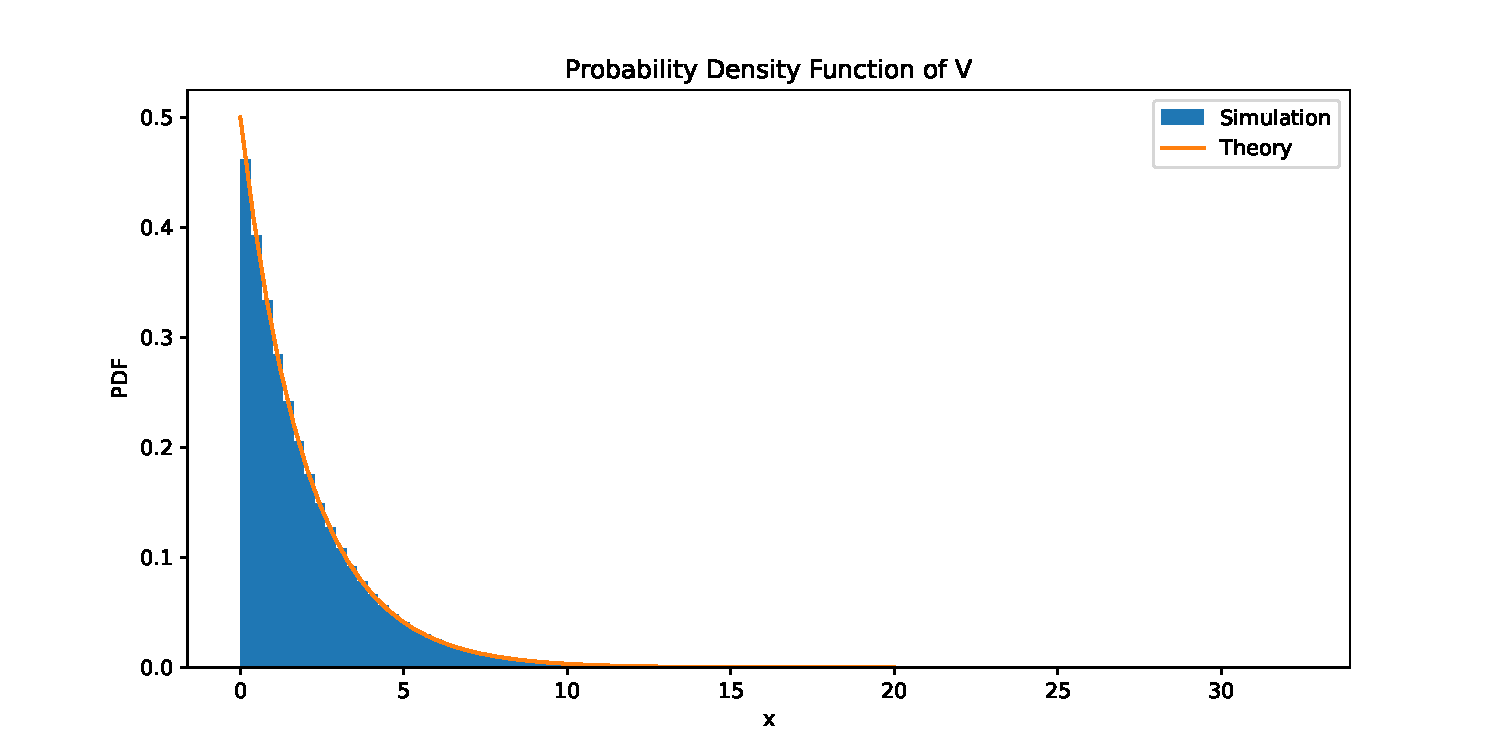
\includegraphics[width=\columnwidth]{./figs/4/4.1.1p.pdf}
\caption{PDF of $V$}
\label{fig:chisq_pdf}
\end{figure}

\item
If
\begin{equation}
F_{V}(x) = 
\begin{cases}
1 - e^{-\alpha x} & x \geq 0 \\
0 & x < 0,
\end{cases}
\label{eq:chisq2_cdf_gen}
\end{equation}
%
find $\alpha$.\\

Let $Z=X^2$ where $X \sim \gauss{0}{1}$. Defining the CDF for $Z$,
\begin{align*}
P_Z(z) &= \pr{Z < z}\\
&= \pr{X^2 < z}\\
&= \pr{-\sqrt{z} < X < \sqrt{z}}\\
&= \int_{-\sqrt{z}}^{\sqrt{z}} p_X(x) ,dx
\end{align*}
Using the derivative of the CDF, the PDF of $Z$ is given by
\begin{align}
\frac{d}{dz}P_Z(z) = p_Z(z)\\
= \frac{p_X(\sqrt{z})+p_X(-\sqrt{z})}{2\sqrt{z}}
\end{align}
Substituting the standard gaussian density function $p_X(x) = \frac{1}{\sqrt{2\pi}}e^{-\frac{x^2}{2}}$, we get
\begin{equation}
p_Z(z) =
\begin{cases}
\frac{1}{\sqrt{2\pi z}}e^{-\frac{z}{2}} & z \ge 0\\
0 & z < 0
\end{cases}
\end{equation}

Now, let $V = X_1^2 + X_2^2$, where $X_1, X_2 \sim \gauss{0}{1}$ are independent. The PDF of $V$ can be obtained by convolution of $p_{X_1^2}(x)$ and $p_{X_2^2}(x)$ is
\begin{align*}
p_V(v) &= p_{X_1^2}(x_1) * p_{X_2^2}(x_2)\\
&= \frac{1}{2\pi} \int_{0}^{v} \frac{e^{-\frac{x}{2}}}{\sqrt{x}}\frac{e^{-\frac{v-x}{2}}}{\sqrt{v-x}} ,dx\\
&= \frac{e^{-\frac{v}{2}}}{2\pi} \int_{0}^{v} \frac{1}{\sqrt{x(v-x)}} ,dx\\
&= \frac{e^{-\frac{v}{2}}}{2\pi} [-\arcsin\left(\frac{v-2x}{v}\right)]0^v\\
&= \frac{e^{-\frac{v}{2}}}{2\pi} \pi\\
&= \frac{e^{-\frac{v}{2}}}{2} \text{ for } v \ge 0
\end{align*}
The CDF of $V$ can be obtained by integrating the PDF:
\begin{align}
	\nonumber
	F_V(v) &= \frac{1}{2} \int_{0}^{v} \exp\left(-\frac{v}{2}\right)&\\
	\label{eq:chisq2_cdf}
	&= 1-\exp\left(-\frac{v}{2}\right) \text{ for } v \ge 0
\end{align}
Comparing \eqref{eq:chisq2_cdf} with \eqref{eq:chisq2_cdf_gen}, $\alpha = \frac{1}{2}$ \\
\begin{center}
\fcolorbox{red}{white}{\parbox{12.5cm}
{\href{https://github.com/Gangagopinath/ASSIGNMENT/tree/main/digitalcommunication/codes/4/4.1.2.py}
{/codes/4/4.1.2.py}}}
\end{center}
 Code shows different values of $\alpha$, and plots it along with the simulated data. The legend in the plot will show which line corresponds to which value of $\alpha$.

\begin{figure}[H]
\centering
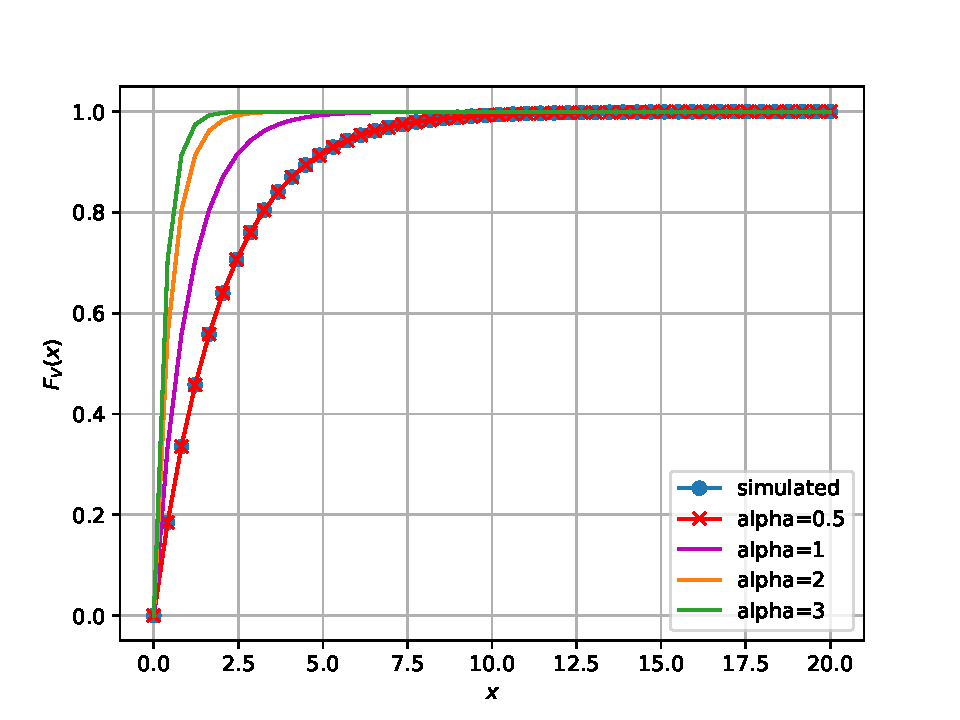
\includegraphics[width=\columnwidth]{./figs/4/4.1.2.pdf}
\caption{CDF of $V$}
\label{fig:cCDF of V }
\end{figure}
\item
\label{ch3_raleigh_sim}
Plot the CDF and PDF of
%
\begin{equation}
A = \sqrt{V}
\end{equation}\\
\solution The CDF and PDF of $A$ are plotted in \figref{fig:sqrt_cdf} and \figref{fig:sqrt_pdf}  using the below code
\begin{center}
\fcolorbox{red}{white}{\parbox{12.5cm}
{\href{https://github.com/Gangagopinath/ASSIGNMENT/tree/main/digitalcommunication/codes/4/4.1.3.py}
{/codes/4/4.1.3.py}}}
\end{center}
\begin{figure}[H]
\centering
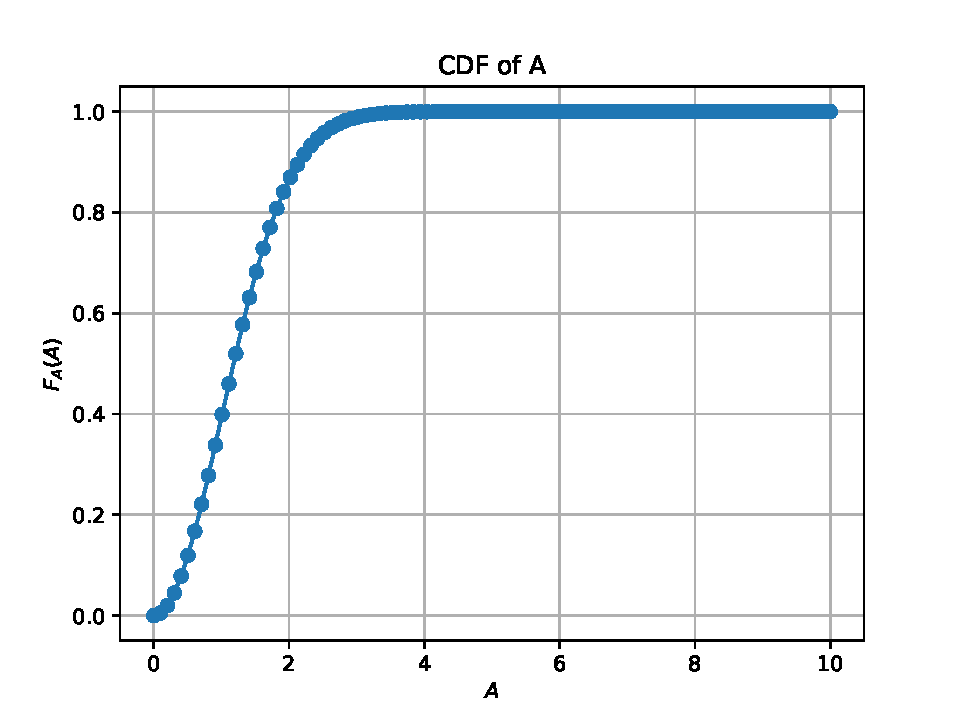
\includegraphics[width=\columnwidth]{./figs/4/4.1.3c.pdf}
\caption{CDF of $V$}
\label{fig:sqrt_cdf}
\end{figure}
\begin{figure}[H]
\centering
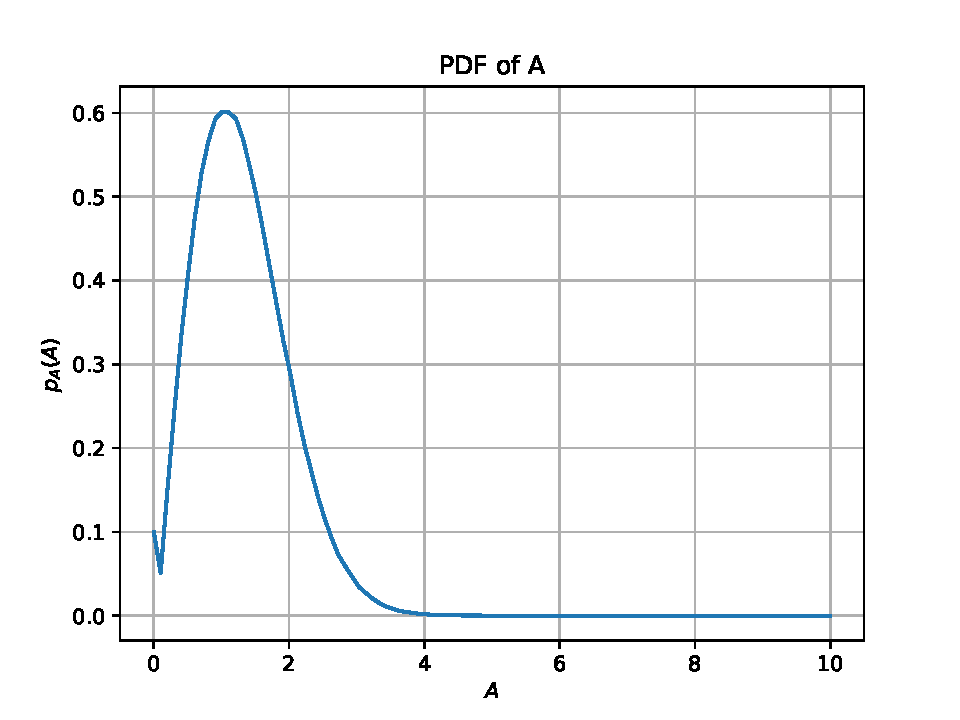
\includegraphics[width=\columnwidth]{./figs/4/4.1.3p.pdf}
\caption{PDF of $V$}
\label{fig:sqrt_pdf}
\end{figure}
\end{enumerate}
\section{Conditional Probability}
\begin{enumerate}
\item
\label{ch4_sim}
Plot 
\begin{equation}
P_e = \pr{\hat{X} = -1|X=1}
\end{equation}
%
for 
\begin{equation}
Y = AX+N,
\end{equation}
where $A$ is Raleigh with $E\sbrak{A^2} = \gamma, N \sim \gauss{0}{1}, X \in \brak{-1,1}$ for $0 \le \gamma \le 10$ dB.\\
\solution
\begin{center}
\fcolorbox{red}{white}{\parbox{12.5cm}
{\href{https://github.com/Gangagopinath/ASSIGNMENT/tree/main/digitalcommunication/codes/4/4.2.1.py}
{/codes/4/4.2.1.py}}}
\end{center}
\begin{figure}[H]
\centering
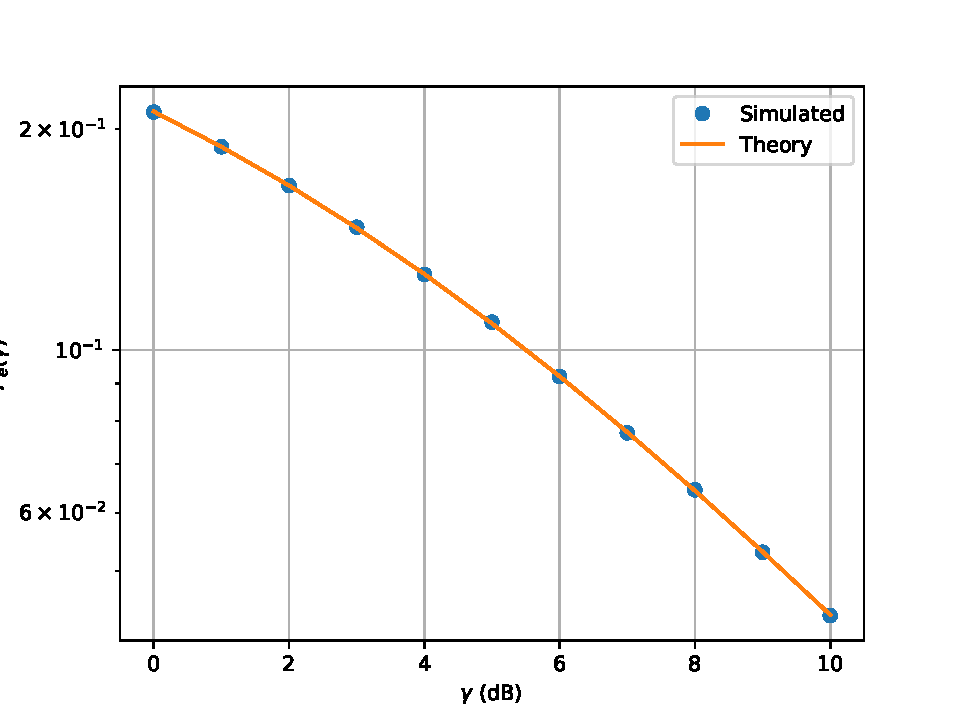
\includegraphics[width=\columnwidth]{./figs/4/4.2.1.pdf}
\caption{$P_e$ versus $\gamma$}
\label{fig:p_e&gamma}
\end{figure}
\item
Assuming that $N$ is a constant, find an expression for $P_e$.  Call this $P_e(N)$\\
\solution The probability of error $P_e$ is given by
\begin{align}
P_e &= \pr{\hat{X} = -1|X=1} \\
&= \pr{Y<0|X=1} \\
&= \pr{AX + N < 0|X=1} \\
&= \pr{A + N < 0} \\
&= \pr{A < -N}.
\end{align}
where $A$ is a Rayleigh random variable with PDF $f_A(x)$.
\begin{align}
f_A(x) = 
\begin{cases}
\frac{x}{\sigma^2}\exp\brak{{-\frac{x^2}{2\sigma^2}}} & x\geq0\\
0 & otherwise
\end{cases}
\end{align}
Now, we need to find the CDF of $A$ at $-N$ to calculate $P_e$, which is given by
\begin{align}
 F_A(-N)&=\int_{-\infty}^{-N} f_A(x)dx\\
&= \int_{0}^{-N} \frac{x}{\sigma^2} \exp\left(-\frac{x^2}{2\sigma^2}\right) dx.\\
 &=1-\exp{\brak{-\frac{N^2}{2\sigma^2}}}
\end{align}
Since $F_A(-N) = 0$ for $N \ge 0$, the final expression for $P_e$ is given by
\begin{equation}
\label{eq:prob_err_bpsk_rayleigh_fN}
P_e(N) = 
\begin{cases}
1-\exp\brak{{-\frac{N^2}{2\sigma^2}}} & N<0\\
0 & otherwise
\end{cases}
\end{equation}
\item
%
\label{ch4_anal}
For a function $g$,
\begin{equation}
E\sbrak{g(X)} = \int_{-\infty}^{\infty}g(x)p_{X}(x)\, dx
\end{equation}
%
Find $P_e = E\sbrak{P_e(N)}$.\\
\solution
Since $N \sim \gauss{0}{1}$ ,
\begin{align}
  p_N(x)= \frac{1}{\sqrt{2\pi}}\exp \brak{-\frac{x^2}{2} }
\end{align}
And from \eqref{eq:prob_err_bpsk_rayleigh_fN} 
\begin{align}
    P_e(x)=
    \begin{cases}
1-\exp\brak{{-\frac{x^2}{2\sigma^2}}} & x<0\\
0 & otherwise
\end{cases}
\end{align}

\begin{align}
 P_e=E\sbrak{P_e(N)} = \int_{-\infty}^{\infty}P_e(x)p_{N}(x)\, dx  
\end{align}
For a Rayleigh Distribution with scale $= \sigma$,
\begin{align}
E\sbrak{A^2} = 2\sigma^2\\
\gamma = 2\sigma^2\\
\end{align}
 Using $P_e(N)$ from \eqref{eq:prob_err_bpsk_rayleigh_fN},
    \begin{align*}
	P_e &= \int_{-\infty}^{\infty} P_e(x)p_N(x) \,dx&\\
		&= \int_{0}^{\infty} \left(1-e^{-\frac{x^2}{2\sigma^2}}\right)\frac{1}{\sqrt{2\pi}}e^{-\frac{x^2}{2}} \,dx\\
	&= \frac{1}{\sqrt{2\pi}}\int_{0}^{\infty} \left(1-e^{-\frac{x^2}{\gamma}}\right)e^{-\frac{x^2}{2}} \,dx\\
	&= \frac{1}{\sqrt{2\pi}}\int_{0}^{\infty} e^{-\frac{x^2}{2}}  \,dx  - \frac{1}{\sqrt{2\pi}}\int_{0}^{\infty} \exp\left(-x^2\left(\frac{1}{\gamma}+\frac{1}{2}\right)\right)  \,dx\\
	&= \frac{1}{2}-\frac{1}{2}\sqrt{\frac{\gamma}{2+\gamma}}
   \end{align*} 
\begin{align}
 P_e = \frac{1}{2} - \frac{1}{2}\sqrt{\frac{\gamma}{2+\gamma}}
\end{align}
\item
Plot $P_e$ in problems \ref{ch4_sim} a nd \ref{ch4_anal} on the same graph w.r.t $\gamma$.  Comment. \\
\solution $P_e$ is plotted w.r.t $\gamma$ in \ref{fig:Pe_gamma1} using the code below.
\begin{center}
\fcolorbox{red}{white}{\parbox{12.5cm}
{\href{https://github.com/Gangagopinath/ASSIGNMENT/tree/main/digitalcommunication/codes/4/4.2.4.py}
{/codes/4/4.2.4.py}}}
\end{center}
\begin{figure}[H]
\centering
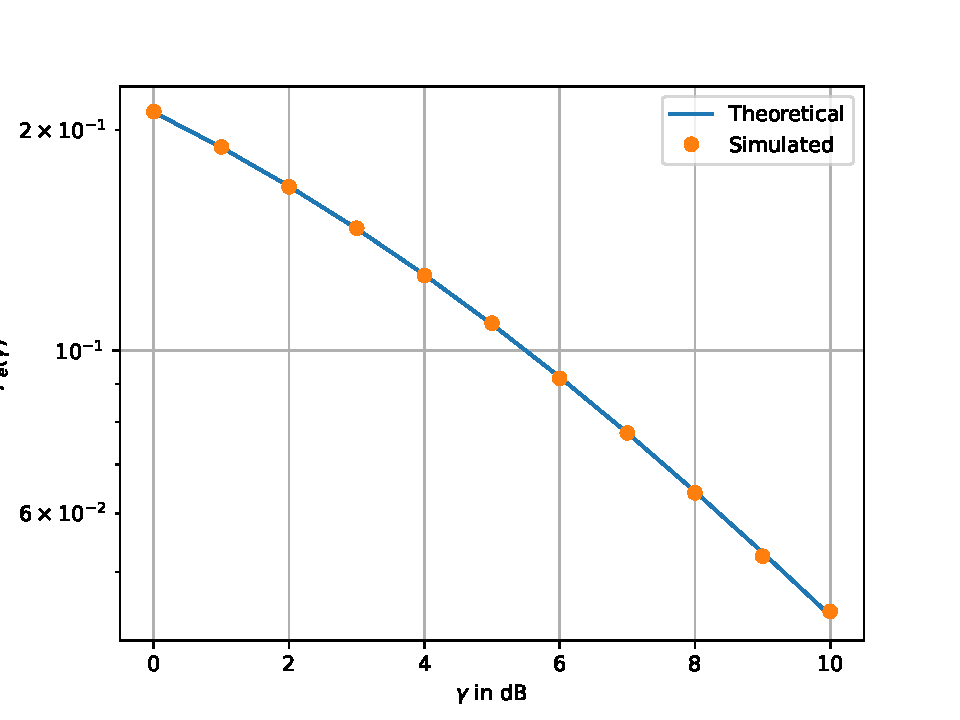
\includegraphics[width=\columnwidth]{./figs/4/4.2.4.pdf}
\caption{The $P_e$ wrt $\gamma$ }
\label{fig:Pe_gamma1}
\end{figure}
\end{enumerate}
\chapter{Bivariate Random Variables: FSK}
\section{Two Dimensions}
Let 
\begin{equation}
\mbf{y} = A\mbf{x} + \mbf{n},
\end{equation}
where 
\begin{align}
x &\in \brak{\mbf{s}_0,\mbf{s}_1}, 
\mbf{s}_0 = 
\begin{pmatrix}
1 
\\
0
\end{pmatrix},
\mbf{s}_1 = 
\begin{pmatrix}
0 
\\
1
\end{pmatrix}
\\
\mbf{n} &= 
\begin{pmatrix}
n_1
\\
n_2
\end{pmatrix},
n_1,n_2 \sim \gauss{0}{1}.
\end{align}
%
\begin{enumerate}
%%
\item
\label{ch5_fsk}
Plot 
%
\begin{equation}
\mbf{y}|\mbf{s}_0 \text{ and } \mbf{y}|\mbf{s}_1
\end{equation}
%
on the same graph using a scatter plot.\\
\begin{center}
\fcolorbox{red}{white}{\parbox{12.5cm}
{\href{https://github.com/Gangagopinath/ASSIGNMENT/tree/main/digitalcommunication/codes/5/5.1.1.py}
{/codes/5/5.1.1.py}}}
\end{center}
\begin{figure}[H]
\centering
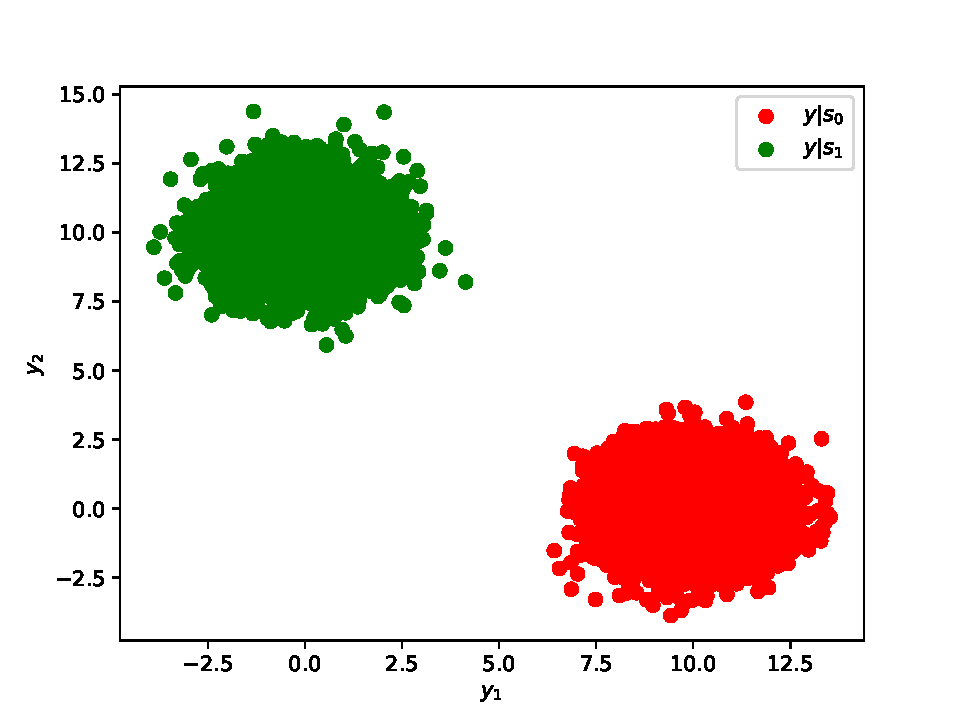
\includegraphics[width=\columnwidth]{./figs/5/5.1.1.pdf}
\caption{Scatter plot of $\mbf{y}|\mbf{s}_0$ and $\mbf{y}|\mbf{s}_1$ }
\label{fig:5.1.1}
\end{figure}
\item
For the above problem, find a decision rule for detecting the symbols $\mbf{s}_0 $ and $\mbf{s}_1$.\\
\solution: 

e decision rule for detecting the symbols $\mbf{s}_0$ and $\mbf{s}_1$ can be expressed mathematically as follows:

Let $\mbf{y} = \begin{bmatrix} y_1 \ y_2 \end{bmatrix}$. Then the decision rule can be written as:
\begin{equation}
y_1 \dec{0}{1} y_2
\label{eq:5.1.2}
\end{equation}

The random vector $\vec{y}|\vec{s}i$ has normally distributed components with PDF:
\begin{equation}
p{\vec{y}|\vec{s}_i}\left(\vec{y}\right) = \frac{1}{2\pi\sqrt{\det{\vec{\Sigma}}}} \exp\left(-\frac{1}{2}\left(\vec{y}-\vec{s}_i\right)^\top \vec{\Sigma}^{-1} \left(\vec{y}-\vec{s}i\right)\right)
\end{equation}
where $\vec{\Sigma}$ is the covariance matrix. With $\vec{\Sigma} = \sigma \vec{I}$, the PDF becomes:
\begin{align}
p{\vec{y}|\vec{s}_i}\left(\vec{y}\right) &= \frac{1}{2 \pi \sigma} \exp\left(-\frac{1}{2 \sigma}\left(\vec{y}-\vec{s}_i\right)^\top \vec{I} \left(\vec{y}-\vec{s}_i\right)\right) \ \\
&= \frac{1}{2 \pi \sigma} \exp\left(-\frac{1}{2 \sigma}\left(\vec{y}-\vec{s}_i\right)^\top \left(\vec{y}-\vec{s}_i\right)\right)
\end{align}

Assuming equal probability for both symbols, we can use the Maximum A Posteriori (MAP) rule to determine the optimum decision. For only two possible symbols, the optimal decision criterion is found by equating $p_{\vec{y}|\vec{s}0}$ and $p{\vec{y}|\vec{s}1}$


\begin{align*}
\log p{\vec{y}|\vec{s}0} &= \log p{\vec{y}|\vec{s}_1} \\
-\frac{1}{2 \sigma}\left(\vec{y}-\vec{s}_0\right)^\top \left(\vec{y}-\vec{s}_0\right) &= -\frac{1}{2 \sigma}\left(\vec{y}-\vec{s}_1\right)^\top \left(\vec{y}-\vec{s}_1\right) \\
\implies \frac{1}{2 \sigma}\left(\vec{y}-\vec{s}_0\right)^\top \left(\vec{y}-\vec{s}_0\right) &= \frac{1}{2 \sigma}\left(\vec{y}-\vec{s}_1\right)^\top \left(\vec{y}-\vec{s}_1\right) \\
\implies \left(\vec{y}-\vec{s}_0\right)^\top \left(\vec{y}-\vec{s}_0\right) &= \left(\vec{y}-\vec{s}_1\right)^\top \left(\vec{y}-\vec{s}_1\right) \\
\implies \left(\vec{y}^\top -\vec{s}_0^\top\right)\left(\vec{y}-\vec{s}_0\right) &= \left(\vec{y}^\top -\vec{s}_1^\top\right)\left(\vec{y}-\vec{s}_1\right) \\
\implies \vec{y}^\top \vec{y} - \vec{y}^\top\vec{s}_0 - \vec{s}_0^\top\vec{y} + \vec{s}_0^\top\vec{s}_0 &= \vec{y}^\top \vec{y} - \vec{y}^\top\vec{s}_1 - \vec{s}_1^\top\vec{y} + \vec{s}_1^\top\vec{s}_1 \\
\implies \vec{s}_0^\top\vec{s}_0 - \vec{s}_1^\top\vec{s}_1 &= 2\vec{y}^\top(\vec{s}_1-\vec{s}_0) - 2\vec{s}_1^\top\vec{y} + 2\vec{s}_0^\top\vec{y} \
\end{align*}
From here, one can obtain the result that $\vec{y} = \frac{\vec{s}_0+\vec{s}_1}{2}$ to satisfy the condition that 

\begin{align*}
\implies \myvec{-1\\1}^\top \vec{y} &= 0
\end{align*}
\item
Plot 
\begin{equation} 
P_e = \pr{\hat{\mbf{x}} = \mbf{s}_1|\mbf{x} = \mbf{s}_0}
\label{eq:5.1.3}
\end{equation}
with respect to the SNR from 0 to 10 dB.\\
\begin{center}
\fcolorbox{red}{white}{\parbox{12.5cm}
{\href{https://github.com/Gangagopinath/ASSIGNMENT/tree/main/digitalcommunication/codes/5/5.1.3.py}
{/codes/5/5.1.3.py}}}
\end{center}
\begin{figure}[H]
\centering
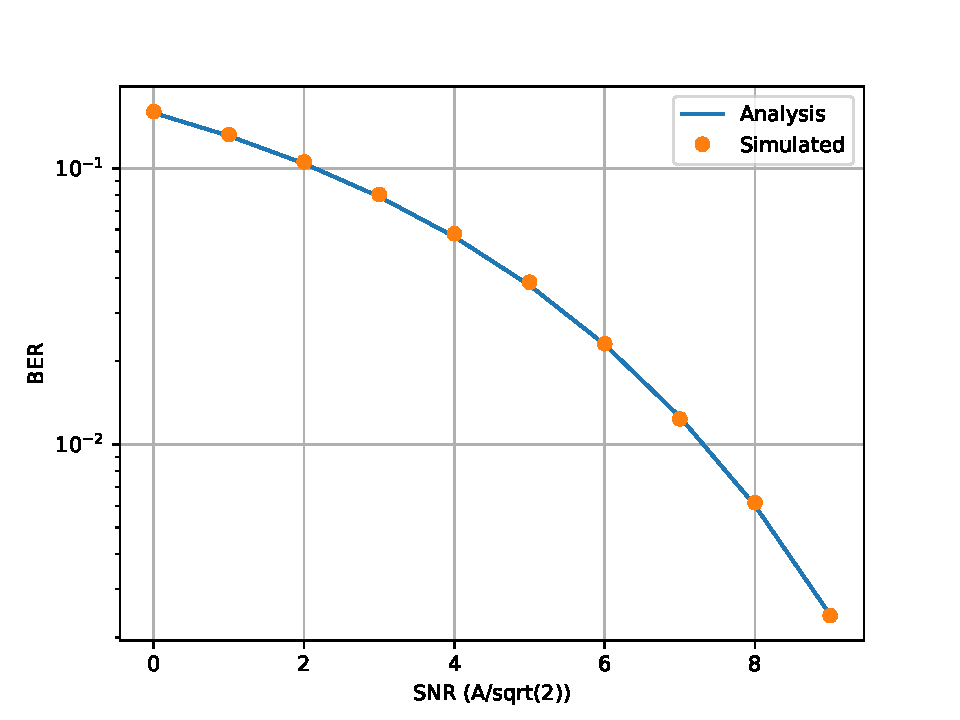
\includegraphics[width=\columnwidth]{./figs/5/5.1.3.pdf}
\caption{$P_e$ versus SNR plot for FSK}
\label{fig:5.1.3}
\end{figure}

\item
Obtain an expression for $P_e$. Verify this by comparing the theory and simulation plots on the same graph.\\
\solution 
The Q-function defined as:

$Q(x) = \frac{1}{\sqrt{2\pi}}\int_{x}^{\infty} e^{-\frac{t^2}{2}} dt$

$P_e$, can be calculated as:
\begin{align*}
P_e &= \text{Pr}(\hat{x}=s_1|x=s_0)\\
& = \text{Pr}(y_1 < y_2|x=s_0)\\
& = \text{Pr}(A + n_1 < n_2)\\
& = \text{Pr}(n_1 - n_2 < -A)  \quad\brak{Z = n_1 - n_2}\\
& = \text{Pr}(Z < -A)      
\end{align*}
Using the properties of normal distributions,$n_1, n_2 \sim \gauss{0}{\sigma^2} ,Z \sim \gauss{0}{2\sigma^2}$.

By changing the inequality sign and using the Q-function, we get:

\begin{align*}
P_e& = \pr{Z < -A} \\
&= \pr{Z > A} \\
&= Q(\frac{A}{\sqrt{2\sigma^2}}) \\
&= Q(\frac{A}{\sqrt{2}})    \quad\brak{\sigma^2 = 1}\\
\end{align*}
Thus, $P_e$ can be represented as the Q-function of $\frac{A}{\sqrt{2}}$
\end{enumerate}
\chapter{Exercises}
\section{BPSK}
\begin{enumerate}
\item
The {\em signal constellation diagram} for BPSK is given by Fig. \ref{fig:6.1}.  The symbols $s_0$ and $s_1$ are equiprobable.  $\sqrt{E_b}$ is the energy transmitted per bit. Assuming a zero mean additive white gaussian noise (AWGN) with variance $\frac{N_0}{2}$,
obtain the symbols that are received\\
\solution The possible received symbols are
\begin{align}
y|s_0 &= \sqrt{E_b} + n
\\
y|s_1 &= -\sqrt{E_b} + n
\end{align}
%
where the AWGN $n \sim \gauss{0}{\frac{N_0}{2}}$.
%%
\begin{figure}[H]
\centering
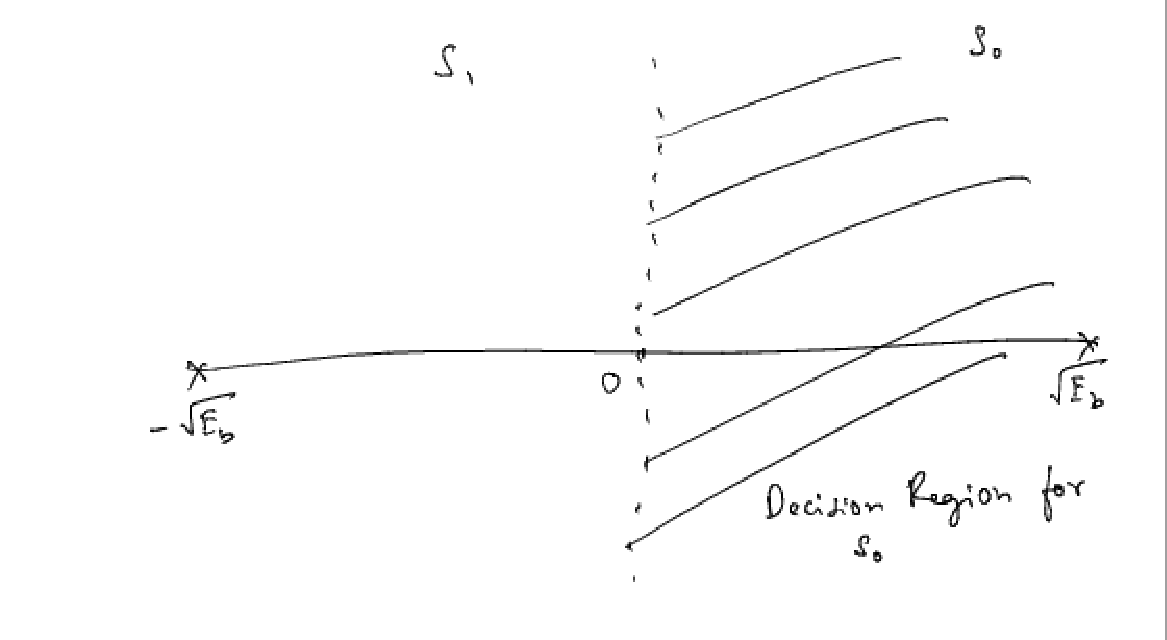
\includegraphics[width=\columnwidth]{./figs/6/1.pdf}
\caption{}
\label{fig:6.1}
\end{figure}
\item
\label{prob:bpsk_decision}
From Fig.\ref{fig:6.1} obtain a decision rule for BPSK
\solution The decision rule is
\begin{equation}
y \dec{s_0}{s_1} 0
\end{equation}
\item
Repeat the previous exercise using the MAP criterion.\\
\solution
\iffalse
The MAP criterion involves calculating the log-likelihood ratio between the received signal being one symbol versus the other symbol and then choosing the symbol that corresponds to the higher log-likelihood ratio.
\fi
The log-likelihood ratios for the two symbols are given by

\begin{align}
\log\frac{p(y|s_0)}{p(y|s_1)} &= \log\frac{\frac{1}{\sqrt{2\pi N_0/2}} \exp\left(-\frac{(y-\sqrt{E_b})^2}{2N_0/2}\right)}{\frac{1}{\sqrt{2\pi N_0/2}} \exp\left(-\frac{(y+\sqrt{E_b})^2}{2N_0/2}\right)} \\
&= \log\exp\left(\frac{2\sqrt{E_b}y}{N_0/2}\right) - \log\left(\exp\left(\frac{2\sqrt{E_b} \sqrt{E_b}}{N_0/2}\right)\right) \\
&= \frac{2\sqrt{E_b}y}{N_0/2} - \frac{2\sqrt{E_b} \sqrt{E_b}}{N_0/2} \\
&= \frac{2\sqrt{E_b}(y-\sqrt{E_b})}{N_0/2}
\end{align}

Therefore, the decision rule based on the MAP criterion is

\begin{equation}
y \dec{s_0}{s_1} \frac{y \sqrt{E_b}}{N_0/2} \gtrless 0
\end{equation}
which is equivalent to the previous decision rule.
\begin{equation}
y \dec{s_0}{s_1} 0
\end{equation}
\item
Using the decision rule in Problem \ref{prob:bpsk_decision}, obtain an expression for the probability of error for BPSK.\\

\solution
Since the symbols are equiprobable, it is sufficient if the error is calculated assuming that a 0 was sent.  This results in
\begin{align}
P_e &= \pr{y < 0|s_0} = \pr{\sqrt{E_b} + n < 0}
\\
&= \pr{ -n > \sqrt{E_b} } = \pr{ n > \sqrt{E_b} }
\label{eq:bpsk_proof_n0}
\end{align}
since $n$ has a symmetric pdf.
Let $w \sim \gauss{0}{1}$.  Then $n = \sqrt{\frac{N_0}{2}}w$. Substituting this in \eqref{eq:bpsk_proof_n0},
\begin{align}
P_e &=  \pr{ \sqrt{\frac{N_0}{2}}w > \sqrt{E_b} } = \pr{ w > \sqrt{\frac{2E_b}{N_0}} }
\\
&= \qfunc{\sqrt{\frac{2E_b}{N_0}}}
\end{align}
%
where $\qfunc{x} \triangleq \pr{w > x}, x \ge 0$.


\item
The PDF of $w \sim \gauss{0}{1}$ is given by
%
\begin{equation}
p_{w}(x) = \frac{1}{\sqrt{2\pi}}\exp\brak{-\frac{x^2}{2}}, -\infty < x < \infty
\end{equation}
and the complementary error function is defined as
\begin{equation}
\operatorname {erfc} (x)={\frac {2}{\sqrt {\pi }}}\int _{x}^{\infty }e^{-t^{2}}\,dt.
\end{equation}
%
Show that 
\begin{equation}
Q(x) = \frac{1}{2}\operatorname {erfc}\left({\frac  {x}{{\sqrt  {2}}}}\right)
\end{equation}\\
\solution
\begin{equation}
Q(a) = \frac{1}{2\pi}\int^{\infty}_{a}e^{-\frac{t^2}{2}},dt
\end{equation}

\begin{align}
a = \frac{a'}{\sqrt{2}},\quad a' = \sqrt{2}a ,\quad
da = \frac{da'}{\sqrt{2}}
\end{align}

Using these substitutions, we can rewrite the equation for $\operatorname{erfc} (x)$ as:

\begin{align}
\operatorname{erfc} (x) &= {\frac {2}{\sqrt {\pi }}}\int _{x}^{\infty }e^{-a^{2}/2},\frac{da'}{\sqrt{2}} \\
&= {\frac {2}{\sqrt {2\pi }}}\int _{\sqrt{2}x}^{\infty }e^{-a^{2}/2},da'\\
\implies \operatorname{erfc} (x) &= 2Q(\sqrt{2}x)\\
\therefore Q(\sqrt{2}x) &= \frac{1}{2}\operatorname{erfc} (x)
\end{align}

So, finally,

\begin{equation}
Q(x) = \frac{1}{2}\operatorname{erfc}\left({\frac {x}{{\sqrt {2}}}}\right)
\end{equation}
\item
Verify the bit error rate (BER) plots for BPSK through simulation and analysis for 0 to 10 dB.
\solution
\begin{center}
\fcolorbox{red}{white}{\parbox{12.5cm}
{\href{https://github.com/Gangagopinath/ASSIGNMENT/tree/main/digitalcommunication/codes/6/6.1.6.py}
{/codes/6/6.1.6.py}}}
\end{center}
\begin{figure}[H]
\centering
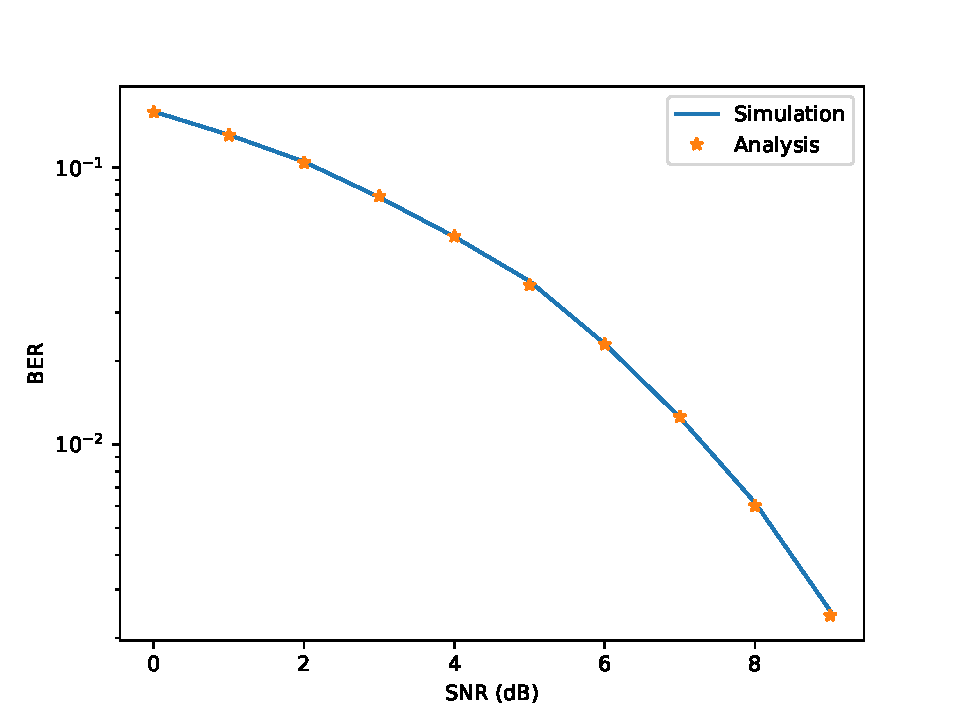
\includegraphics[width=\columnwidth]{./figs/6/6.1.6.pdf}
\caption{}
\label{fig:6.1.6}
\end{figure}
\item
\label{prob:craigs_formula_proof}
Show that
\begin{equation}
Q(x) = \frac{1}{\pi}\int^{\frac{\pi}{2}}_{0}e^{-\frac{x^2}{2\sin^2 \theta}}\,d\theta
\end{equation}\\
\solution
The Gaussian Q‐function, which is defined by
\begin{align*}
Q(x) &= \int_{x}^{\infty} f_{u}(u) \,du \\
&=\frac{1}{2\pi }\int_{u}^{\infty}e^{-\frac{u}{2}}\\
&=\frac{1}{2\pi}\int_{z}^{\infty}\int_{-\infty}^{\infty} \exp\left(-\frac{u^2+v^2}{2}\right) \,du\,dv\\
\label{eq:qfunc_biv_integ}
\end{align*}
Transforming the  Cartesian coordinates in \eqref{eq:qfunc_biv_integ} to polar coordinates as $u= rsin\theta, v=rcos\theta$ and $du dv=r dr d\theta$ 
\begin{align*}
	Q(x) &= \frac{1}{2\pi}\int_{0}^{\pi} d\theta \int_{\frac{x}{\sin\theta}}^{\infty} \exp\left(-\frac{r^2}{2}\right)r \,dr\ \\
&= \frac{1}{2\pi}\int_{0}^{\pi} \exp\left(-\frac{x^2}{2\sin^2\theta}\right) \,d\theta\\
	&= \frac{1}{\pi}\int_{0}^{\frac{\pi}{2}} \exp\left(-\frac{x^2}{2\sin^2\theta}\right) \,d\theta 
\end{align*}
\end{enumerate}
\section{Coherent BFSK}
\begin{enumerate}
\item
The signal constellation for binary frequency shift keying (BFSK) is given in \figref{fig:bfsk_const}.
Obtain the equations for the received symbols.
\begin{figure}[H]
\centering
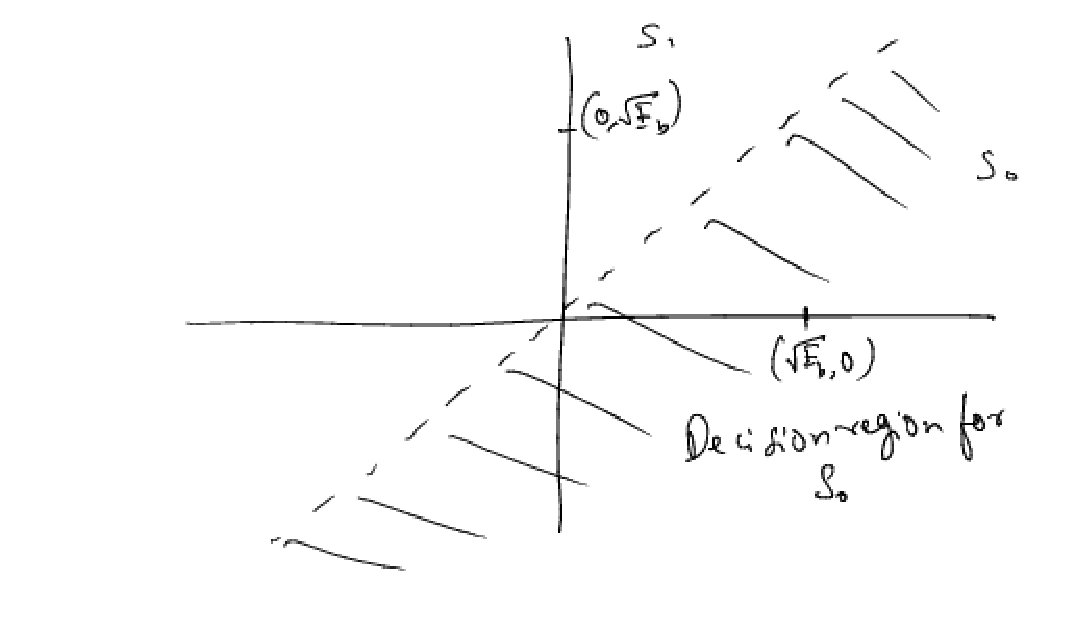
\includegraphics[width=\columnwidth]{./figs/6/2.pdf}
\caption{}
\label{fig:bfsk_const}
\end{figure}
\solution
The received symbols are given by
\begin{align}
\mathbf{y}|s_0 = 
\myvec{
\sqrt{E_b} \\
0
}
+
\myvec{
 n_{1}\\
n_{2}
},
\end{align}
and 
\begin{align}
\mathbf{y}|s_1 = 
\myvec{
0\\
\sqrt{E_b} 
}
+
\myvec{
n_{1}\\
 n_{2}
},
\end{align}
where $n_1,n_2 \sim \gauss{0}{\frac{N_0}{2}}$. and
$
\mathbf{y} = 
\myvec{
y_{1}\\
 y_{2}
}
$.
\item
Obtain a decision rule for BFSK from \figref{fig:bfsk_const}.

\solution The decision rule is
\begin{equation}
y_1 \dec{s_0}{s_1} y_2
\end{equation}
\item
Repeat the previous exercise using the MAP criterion.\\
\solution
The Maximum A Posteriori (MAP) criterion for deciding the symbol $s$ from the received signal $\mathbf{y}$ can be given as:

\begin{equation}
s = \arg\max_{s_0,s_1} P(s|\mathbf{y})
\end{equation}

The likelihood function can be given as:

\begin{align}
P(\mathbf{y}|s_0) &= \frac{1}{\sqrt{2\pi \frac{N_0}{2}}} \exp \left(-\frac{||\mathbf{y} - \mathbf{y}|s_0||^2}{2\frac{N_0}{2}}\right) \\
P(\mathbf{y}|s_1) &= \frac{1}{\sqrt{2\pi \frac{N_0}{2}}} \exp \left(-\frac{||\mathbf{y} - \mathbf{y}|s_1||^2}{2\frac{N_0}{2}}\right)
\end{align}

where $||\cdot||$ represents the Euclidean distance.

Assuming equal prior probabilities for both symbols, i.e., $P(s_0) = P(s_1) = \frac{1}{2}$, the decision rule using the MAP criterion can be given as:

\begin{equation}
s = \arg\max_{s_0,s_1} \frac{1}{\sqrt{2\pi \frac{N_0}{2}}} \exp \left(-\frac{||\mathbf{y} - \mathbf{y}|s||^2}{2\frac{N_0}{2}}\right)
\end{equation}

can be represented as:

\begin{equation}
y_1 \dec{s_0}{s_1} y_2
\end{equation}
 The decision is made by comparing the values of $y_1$ and $y_2$ and choosing the symbol with the highest likelihood of being transmitted, given the received signal.

 \end{enumerate}
\end{document}